% Author: Daniel Vartanian.
% Licence: MIT. See <https://opensource.org/license/mit/> to learn more.
% Based on: template.tex, developed by the Quarto team and
%   abtex2-modelo-trabalho-academico.tex, v-1.9.7, developed by
%   Lauro César Araujo and the team behind abnt2tex, with additional guidance
%   from the theses and dissertations regulations of the University of São Paulo
%   (USP). For more information, please visit <http://www.abntex.net.br/>.

% For help, see:
% * <https://quarto.org/docs/reference/formats/pdf.html>
% * <https://github.com/abntex/abntex2/wiki/ComoCustomizar>
% * <https://www.ctan.org/pkg/abntex2>
% * <https://www.ctan.org/pkg/memoir>
% * <https://www.ctan.org/pkg/hyperref>

% TODO:
% * Slightly move the toc to the left, in a way that the spacing between titles
%   and numbers become the same as the textual chapters.
% * Remove the hyperlink in the section numbering within TOC.
% * Remove hiperlink spans by page breaks. See: <https://tex.stackexchange.com/questions/54136/hyperref-link-spans-a-pagebreak-looks-ugly>.

% -----
% Preamble
% -----

\PassOptionsToPackage{
unicode
}{hyperref}

\PassOptionsToPackage{hyphens}{url}

\PassOptionsToPackage{dvipsnames,svgnames,x11names}{xcolor}


\documentclass[
12pt,
openright,
oneside,
a4paper,
chapter=TITLE,
section=TITLE,
french,
spanish,
brazil,
english
]{abntex2}\usepackage{array}
\usepackage{booktabs}
\usepackage{calc}
\usepackage{caption}
\usepackage{color}
\usepackage{colortbl}
\usepackage{amsmath}
\usepackage{amssymb}
\usepackage{booktabs}
\usepackage{enumitem}
\usepackage{etoolbox}
\usepackage{float}
\usepackage[T1]{fontenc}
\usepackage[hang]{footmisc}
\usepackage{graphicx}
\usepackage{iftex}
\usepackage{indentfirst}
\usepackage[utf8]{inputenc}
\usepackage{lastpage}
\usepackage{lipsum}
\usepackage{longtable}
\usepackage{microtype}
\usepackage{multirow}
\usepackage{parskip}
\usepackage{pdfpages}
\usepackage[table]{xcolor}

\usepackage{hyperref}

\ifPDFTeX
  \usepackage{textcomp} % provide euro and other symbols
\else % if luatex or xetex
  \usepackage{unicode-math}
\fi\newlength{\microskipamount}
\newlength{\tinyskipamount}
\newlength{\hugeskipamount}

\setlength{\microskipamount}{0.25\baselineskip} % Arial/12pt/1.5 == 5.4375pt
\setlength{\tinyskipamount}{0.5\baselineskip} % Arial/12pt/1.5 == 10.875pt
\setlength{\smallskipamount}{0.75\baselineskip} % Arial/12pt/1.5 == 16.3125pt
\setlength{\medskipamount}{1\baselineskip} % Arial/12pt/1.5 == 21.75pt
\setlength{\bigskipamount}{1.5\baselineskip} % Arial/12pt/1.5 == 32.625pt
\setlength{\hugeskipamount}{2\baselineskip }% Arial/12pt/1.5 == 43.5pt

\newcommand{\microskip}{\vspace{\microskipamount}}
\newcommand{\tinyskip}{\vspace{\tinyskipamount}}
\newcommand{\hugeskip}{\vspace{\hugeskipamount}}

\setlength{\beforechapskip}{\bigskipamount}
\setlength{\afterchapskip}{\smallskipamount}
\setbeforesecskip{\medskipamount}
\setaftersecskip{\smallskipamount}
\setbeforesubsecskip{\medskipamount}
\setaftersubsecskip{\smallskipamount}
\setbeforesubsubsecskip{\medskipamount}
\setaftersubsubsecskip{\smallskipamount}
\setbeforeparaskip{\medskipamount}
\setafterparaskip{0\smallskipamount}
% \setparahook{\addvspace{\smallskipamount}}% Set page -----

\setlength{\headsep}{1cm}
\setlength{\footskip}{1cm}
\checkandfixthelayout

% Set text spacing -----

\renewcommand{\familydefault}{\sfdefault}

\renewcommand{\baselinestretch}{1.5}

\setlength{\parindent}{1cm}

\setlength{\parskip}{0ex}

% Set text font -----


\ifPDFTeX\else
    % xetex/luatex font selection
  \setmainfont[]{Arial}
  \setsansfont[]{Arial}
  \setmonofont[ItalicFont=FragmentMono-Italic.otf,Scale=0.75]{FragmentMono-Regular.otf}




\fi


% Set footnote -----

\setlength{\footnotemargin}{0.5em} % Equal to `\footmarkwidth`
\let\svfootnoterule\footnoterule % Equal to `\footmarksep`
\renewcommand\footnoterule{\svfootnoterule\vspace{1ex}}\newcommand{\capaname}{Capa}
\newcommand{\fichacatalograficaname}{Ficha catalográfica}
\newcommand{\resumoestrangeironame}{Resumo}
\newcommand{\glossarioname}{Glossário}

\addto\captionsenglish{
  \renewcommand{\capaname}{Cover}
  \renewcommand{\folhaderostoname}{Title page}
  \renewcommand{\fichacatalograficaname}{Cataloging record}
  \renewcommand{\errataname}{Errata}
  \renewcommand{\folhadeaprovacaoname}{Approval sheet}
  \renewcommand{\dedicatorianame}{Inscription}
  \renewcommand{\agradecimentosname}{Acknowledgements}
  \renewcommand{\epigraphname}{Epigraph}
  \renewcommand{\resumoname}{Abstract}
  \renewcommand{\resumoestrangeironame}{Resumo}
  \renewcommand{\listfigurename}{List of figures}
  \renewcommand{\listtablename}{List of tables}
  \renewcommand{\listadesiglasname}{List of abbreviations and acronyms}
  \renewcommand{\listadesimbolosname}{List of symbols}
  \renewcommand{\contentsname}{Contents}
  \renewcommand{\bibname}{References}
  \renewcommand{\glossarioname}{Glossary}
  \renewcommand{\apendicename}{APPENDIX}
  \renewcommand{\apendicesname}{Appendices}
  \renewcommand{\anexoname}{ANNEX}
  \renewcommand{\anexosname}{Annexes}
  \renewcommand{\indexname}{Index}
  \renewcommand{\orientadorname}{Supervisor:}
  \renewcommand{\coorientadorname}{Co-supervisor:}
  \renewcommand{\fontename}{Source}
  \renewcommand{\notaname}{Note}
  \renewcommand{\pageautorefname}{page}
  \renewcommand{\sectionautorefname}{section}
  \renewcommand{\subsectionautorefname}{subsection}
  \renewcommand{\subsubsectionautorefname}{subsubsection}
  \renewcommand{\paragraphautorefname}{subsubsubsection}
}

\addto\captionsbrazil{
  \renewcommand{\capaname}{Capa}
  \renewcommand{\folhaderostoname}{Folha de rosto}
  \renewcommand{\fichacatalograficaname}{Ficha catalográfica}
  \renewcommand{\errataname}{Errata}
  \renewcommand{\folhadeaprovacaoname}{Folha de aprovação}
  \renewcommand{\dedicatorianame}{Dedicatória}
  \renewcommand{\agradecimentosname}{Agradecimentos}
  \renewcommand{\epigraphname}{Epígrafe}
  \renewcommand{\resumoname}{Resumo}
  \renewcommand{\resumoestrangeironame}{Abstract}
  \renewcommand{\listfigurename}{Lista de figuras}
  \renewcommand{\listtablename}{Lista de tabelas}
  \renewcommand{\listadesiglasname}{Lista de abreviaturas e siglas}
  \renewcommand{\listadesimbolosname}{Lista de símbolos}
  \renewcommand{\contentsname}{Sumário}
  \renewcommand{\bibname}{Referências}
  \renewcommand{\glossarioname}{Glossário}
  \renewcommand{\apendicename}{APÊNDICE}
  \renewcommand{\apendicesname}{Apêndices}
  \renewcommand{\anexoname}{ANEXO}
  \renewcommand{\anexosname}{Anexos}
  \renewcommand{\indexname}{Índice}
  \renewcommand{\orientadorname}{Asesor:}
  \renewcommand{\coorientadorname}{Coasesor:}
  \renewcommand{\sourcename}{Fuente}
  \renewcommand{\notaname}{Nota}
  \renewcommand{\pageautorefname}{página}
  \renewcommand{\sectionautorefname}{sección}
  \renewcommand{\subsectionautorefname}{subsección}
  \renewcommand{\subsubsectionautorefname}{subsubsección}
  \renewcommand{\paragraphautorefname}{subsubsubsección}
}

\addto\captionsspanish{
  \renewcommand{\capaname}{Portada}
  \renewcommand{\folhaderostoname}{Página de título}
  \renewcommand{\fichacatalograficaname}{Ficha catalográfica}
  \renewcommand{\errataname}{Errata}
  \renewcommand{\folhadeaprovacaoname}{Hoja de aprobación}
  \renewcommand{\dedicatorianame}{Dedicatoria}
  \renewcommand{\agradecimentosname}{Agradecimientos}
  \renewcommand{\epigraphname}{Epígrafe}
  \renewcommand{\resumoname}{Resumen}
  \renewcommand{\resumoestrangeironame}{Resumo}
  \renewcommand{\listfigurename}{Lista de figuras}
  \renewcommand{\listtablename}{Lista de tablas}
  \renewcommand{\listadesiglasname}{Lista de abreviaturas y siglas}
  \renewcommand{\listadesimbolosname}{Lista de símbolos}
  \renewcommand{\contentsname}{Sumario}
  \renewcommand{\bibname}{Referencias}
  \renewcommand{\glossarioname}{Glosario}
  \renewcommand{\apendicename}{APÉNDICE}
  \renewcommand{\apendicesname}{Apéndices}
  \renewcommand{\anexoname}{ANEXO}
  \renewcommand{\anexosname}{Anexos}
  \renewcommand{\indexname}{Índice}
  \renewcommand{\orientadorname}{Asesor:}
  \renewcommand{\coorientadorname}{Coasesor:}
  \renewcommand{\sourcename}{Fuente}
  \renewcommand{\notaname}{Nota}
  \renewcommand{\pageautorefname}{página}
  \renewcommand{\sectionautorefname}{sección}
  \renewcommand{\subsectionautorefname}{subsección}
  \renewcommand{\subsubsectionautorefname}{subsubsección}
  \renewcommand{\paragraphautorefname}{subsubsubsección}
}

\addto\captionsfrench{
  \renewcommand{\capaname}{Couverture}
  \renewcommand{\folhaderostoname}{Page de titre}
  \renewcommand{\fichacatalograficaname}{Fiche cataloguée}
  \renewcommand{\errataname}{Errata}
  \renewcommand{\folhadeaprovacaoname}{Feuille d'approbation}
  \renewcommand{\dedicatorianame}{Dédiace
  \renewcommand{\agradecimentosname}{Remerciements}}
  \renewcommand{\epigraphname}{Épigraphe}
  \renewcommand{\resumoname}{Résumé}
  \renewcommand{\resumoestrangeironame}{Resumo}
  \renewcommand{\listfigurename}{Liste des figures}
  \renewcommand{\listtablename}{Liste des tableaux}
  \renewcommand{\listadesiglasname}{Liste des abréviations et sigles}
  \renewcommand{\listadesimbolosname}{Liste des symboles}
  \renewcommand{\contentsname}{Sommaire}
  \renewcommand{\bibname}{Références}
  \renewcommand{\glossarioname}{Glossaire}
  \renewcommand{\apendicename}{APPENDICE}
  \renewcommand{\apendicesname}{Appendices}
  \renewcommand{\anexoname}{ANNEXE}
  \renewcommand{\anexosname}{Annexes}
  \renewcommand{\indexname}{Index}
  \renewcommand{\orientadorname}{Conseiller:}
  \renewcommand{\coorientadorname}{Co-conseiller:}
  \renewcommand{\sourcename}{Source}
  \renewcommand{\notaname}{Note}
  \renewcommand{\pageautorefname}{page}
  \renewcommand{\sectionautorefname}{section}
  \renewcommand{\subsectionautorefname}{sous-section}
  \renewcommand{\subsubsectionautorefname}{sous-sous-section}
  \renewcommand{\paragraphautorefname}{sous-sous-sous-section}
}% See `babel.tex` for language changes.
% See `toc.text` for changes related to the ToC.

% Set page numbering -----

\makepagestyle{abntheadings}
\makeevenhead{abntheadings}{\ABNTEXfontereduzida\thepage}{}{}
\makeoddhead{abntheadings}{}{}{\ABNTEXfontereduzida\thepage}

% Set text variables -----

\renewcommand{\ABNTEXpartfont}{\normalfont\bfseries}
\renewcommand{\ABNTEXpartfontsize}{\normalsize}
\renewcommand{\ABNTEXchapterfont}{\normalfont\bfseries}
\renewcommand{\ABNTEXchapterfontsize}{\normalsize}
\renewcommand{\ABNTEXsectionfont}{\normalfont}
\renewcommand{\ABNTEXsectionfontsize}{\normalsize}
\renewcommand{\ABNTEXsubsectionfont}{\normalfont\bfseries}
\renewcommand{\ABNTEXsubsectionfontsize}{\normalsize}
\renewcommand{\ABNTEXsubsubsectionfont}{\normalfont}
\renewcommand{\ABNTEXsubsubsectionfontsize}{\normalsize}
\renewcommand{\ABNTEXsubsubsubsectionfont}{\normalfont}
\renewcommand{\ABNTEXsubsubsubsectionfontsize}{\normalsize\itshape}
\renewcommand{\ABNTEXfontereduzida}{\footnotesize}
\renewcommand{\ABNTEXcaptiondelim}{~\textendash~}
\renewcommand{\ABNTEXcaptionfontedelim}{:~}

\renewcommand{\captiontitlefont}{\ABNTEXfontereduzida}

% Set new commands -----

\providecommand{\imprimiruniversidade}{}
\newcommand{\universidade}[1]{\renewcommand{\imprimiruniversidade}{#1}}

\providecommand{\imprimirescola}{}
\newcommand{\escola}[1]{\renewcommand{\imprimirescola}{#1}}

\providecommand{\imprimirprograma}{}
\newcommand{\programa}[1]{\renewcommand{\imprimirprograma}{#1}}

\newcommand{\imprimirtipodetrabalho}{\imprimirtipotrabalho}

\providecommand{\imprimirtipodetituloacademico}{}
\newcommand{\tipodetituloacademico}[1]{\renewcommand{\imprimirtipodetituloacademico}{#1}}

\providecommand{\imprimirtituloacademico}{}
\newcommand{\tituloacademico}[1]{\renewcommand{\imprimirtituloacademico}{#1}}

\providecommand{\imprimirareadeconcentracao}{}
\newcommand{\areadeconcentracao}[1]{\renewcommand{\imprimirareadeconcentracao}{#1}}

\providecommand{\imprimirnotadeversao}{}
\newcommand{\notadeversao}[1]{\renewcommand{\imprimirnotadeversao}{#1}}

% Set chapter style -----

\renewcommand{\chapnamefont}{\normalfont\normalsize}
\renewcommand{\chapnumfont}{\normalfont\normalsize}

\setsecnumformat{\chapnumfont\csname the#1\endcsname\quad}

\renewcommand{\printchaptername}{
  \ifthenelse{\boolean{abntex@apendiceousecao}}{
    \chapnamefont \ABNTEXchapterupperifneeded{\appendixname} % [Changed]
  }{}
}

% Open an issue about it (`\hspace{-1em}`) - Title streching.
\renewcommand{\chapternamenum}{
  \ifthenelse{\boolean{abntex@apendiceousecao}}{
    \hspace{-2em} \space
  }{}
}

\renewcommand{\printchapternum}{
  \tocprintchapter
  \setboolean{abntex@innonumchapter}{false}
  \chapnumfont
  \thechapter % [Changed]
  % \ifthenelse{\boolean{abntex@apendiceousecao}}{ % [Removed]
  %   \tocinnonumchapter
  %   \ABNTEXcaptiondelim
  % }{}
}

\renewcommand{\afterchapternum}{
  \ifthenelse{\boolean{abntex@apendiceousecao}}{ % [Added]
    \normalfont \hspace{-1em} \space\ABNTEXcaptiondelim\space \hspace{-1.5em}
  }{
    \hspace{-0.875em}
  }
}

\renewcommand{\printchapternonum}{
  \tocprintchapternonum
  \setlength{\afterchapskip}{\hugeskipamount} % [Added]
  \setboolean{abntex@innonumchapter}{true}
}

\renewcommand{\printchaptertitle}[1]{
  \chaptitlefont
  \ifthenelse{\boolean{abntex@innonumchapter}}{
    \centering \ABNTEXchapterupperifneeded{#1}
  }{
    \ifthenelse{\boolean{abntex@apendiceousecao}}{
      \normalfont \ABNTEXchapterupperifneeded{#1}
    }{
      \ABNTEXchapterupperifneeded{#1}
    }
  }
}

% Set `\textual` -----

\renewcommand{\textual}{
  \pagestyle{abntheadings}
  \aliaspagestyle{chapter}{abntheadings}
}

% Set cover -----

\renewcommand{\imprimircapa}{
  \phantomsection\pdfbookmark[0]{\capaname}{}
  \begin{capa}%
  \begin{adjustwidth}{-1cm}{0cm}
  \center
  \imprimirinstituicao

  \vfill
  \imprimirautor

  \vfill
  \textbf{\imprimirtitulo}

  \vfill
  \vspace{6.5cm}
  \imprimirlocal

  \imprimirdata
  \vspace{1.5cm}
  \end{adjustwidth}
  \end{capa}
}

% Set title page -----

\makeatletter
\renewcommand{\folhaderostocontent}{
  \begin{center}
  \imprimirautor

  \vfill
  \bfseries\imprimirtitulo

  \vfill
  \bfseries\imprimirnotadeversao\normalfont

  \vfill
  \abntex@ifnotempty{
    \imprimirpreambulo
  }{
    \hspace{0.35\textwidth}
    \begin{minipage}{.6\textwidth}
    \SingleSpacing
    \imprimirpreambulo
    \end{minipage}
  }

  \vfill
  \imprimirlocal

  \imprimirdata
  \vspace{1cm}
  \end{center}
}
\makeatother

% Set cataloging record -----

\renewenvironment{fichacatalografica}{
  \PRIVATEbookmarkthis{\fichacatalograficaname}
  \setlength{\parindent}{0cm}
  \begin{SingleSpacing}
}{
  \end{SingleSpacing}
}

% Set errata -----

\renewenvironment{errata}[1][\errataname]{
  \newpage
  \phantomsection
  \pretextualchapter{#1}
}{
  \cleardoublepage
}

% Set approval sheet -----

\renewenvironment{folhadeaprovacao}[1][\folhadeaprovacaoname]{
  \clearpage
  \PRIVATEbookmarkthis{#1}
  \setlength\parindent{0cm}
  \AtBeginEnvironment{tabular}{\normalsize}
  \begin{SingleSpace}
}{
  \end{SingleSpace}
  \cleardoublepage
}

% Set abstract -----

\newenvironment{resumoenv}[1][\resumoname]{
  \pretextualchapter{#1}
  \begingroup
  \setlength{\parindent}{0cm}
  \setlength{\parskip}{\smallskipamount} % The troublemaker.
  \AtBeginEnvironment{tabular}{\normalsize}
  \renewcommand{\arraystretch}{1}
  \setlength{\aboverulesep}{0ex}
  \setlength{\belowrulesep}{0ex}
  \setlength{\arrayrulewidth}{0pt}
  \setlength{\tabcolsep}{0cm}
  \vspace{-\smallskipamount} % !
  \begin{SingleSpace}
}{
  \end{SingleSpace}
  \cleardoublepage
  \endgroup
}

% Set list of abbreviations and acronyms -----

\renewenvironment{siglas}{
  \pretextualchapter{\listadesiglasname}
}{
  \cleardoublepage
}

% Set list of symbols -----

\renewenvironment{simbolos}{
  \pretextualchapter{\listadesimbolosname}
}{
  \cleardoublepage
}

% Set glossary -----

\newenvironment{glossario}{
  \tocprintchapternonum
}{
  \cleardoublepage
}

% Set appendices and annexes -----

\renewcommand{\PRIVATEapendiceconfig}[2]{
  \setboolean{abntex@apendiceousecao}{true}
  \renewcommand{\appendixname}{#1}
  \renewcommand{\apendicesname}{#1}

  \ifthenelse{\boolean{ABNTEXsumario-abnt-6027-2012}}{
    \renewcommand{\appendixtocname}{\uppercase{#2}}
  }{
    \renewcommand{\appendixtocname}{#2}
  }

  \renewcommand{\appendixpagename}{#2}
  \renewcommand{\appendixtocname}{#2}
  % \switchchapname{#1} % [Altered]
  \renewcommand{\cftappendixname}{} % [Altered]
  \tocpartapendices % [Added]

  % Note:
  %
  % \cleardoublepage
  % \phantomsection
  % \addcontentsline{toc}{part}{Appendices}
  % \appendix
  %
  % is automatically add by the Quarto render.
}

\renewcommand{\apendices}{
  \PRIVATEapendiceconfig{\apendicename}{\apendicesname}
  \appendix
}

\renewenvironment{apendicesenv}{
  \PRIVATEapendiceconfig{\apendicename}{\apendicesname}
  \begin{appendix}
}{
  \end{appendix}
  \setboolean{abntex@apendiceousecao}{false}
  \bookmarksetup{startatroot}
}

\renewcommand{\anexos}{
  % \cftinserthook{toc}{AAA} [Removed]
  \PRIVATEapendiceconfig{\anexoname}{\anexosname}

  \newpage % [Added]
  \phantomsection % [Added]
  \addcontentsline{toc}{part}{\appendixtocname} % [Added]

  \appendix
  \renewcommand\theHchapter{anexochapback.\arabic{chapter}}
}

\renewenvironment{anexosenv}{
  \PRIVATEapendiceconfig{\anexoname}{\anexosname}

  \newpage % [Added]
  \phantomsection % [Added]
  \addcontentsline{toc}{part}{\appendixtocname} % [Added]

  \begin{appendix}
  \renewcommand\theHchapter{anexochapback.\arabic{chapter}}
}{
  \end{appendix}
  \setboolean{abntex@apendiceousecao}{false}
  \bookmarksetup{startatroot}
}\definecolor{blue}{HTML}{2905C3}

% See <https://getbootstrap.com/docs/4.0/utilities/colors/>.
\definecolor{quarto-blue}{HTML}{2780E3}
\definecolor{quarto-lighter-blue}{HTML}{ECF4FC}
\definecolor{quarto-orange}{HTML}{FF7518}
\definecolor{quarto-ligther-orange}{HTML}{FFF3EB}
\definecolor{quarto-red}{HTML}{D9534F}
\definecolor{quarto-ligther-red}{HTML}{FCF1F1}
\definecolor{quarto-green}{HTML}{3FB618}
\definecolor{quarto-ligther-green}{HTML}{EFF9EB}
\definecolor{quarto-purple}{HTML}{7D12BA}
\definecolor{quarto-gray}{HTML}{A3A3A3}
\definecolor{quarto-medium-gray}{HTML}{CFD0D1}
\definecolor{quarto-ligther-gray}{HTML}{F1F3F5}

\definecolor{bs-link-color}{HTML}{39729E}% \usepackage{graphicx}
\makeatletter
\def\maxwidth{\ifdim\Gin@nat@width>\linewidth\linewidth\else\Gin@nat@width\fi}
\def\maxheight{\ifdim\Gin@nat@height>\textheight\textheight\else\Gin@nat@height\fi}
\makeatother

% Scale images if necessary, so that they will not overflow the page
% margins by default, and it is still possible to overwrite the defaults
% using explicit options in \includegraphics[width, height, ...]{}
\setkeys{Gin}{width=\maxwidth,height=\maxheight,keepaspectratio}

% Set default figure placement to htbp
\makeatletter
\def\fps@figure{htbp}
\makeatother

\makeatletter
\setlength{\@fptop}{5pt} % Set distance from top of page to first float
\makeatother

% Set captions and legends -----

\DeclareCaptionFont{ABNTEXfontereduzida}{\ABNTEXfontereduzida}

\captionsetup{
  font=ABNTEXfontereduzida,
  justification=centering
}

\renewcommand{\abovecaptionskip}{\tinyskipamount}
\renewcommand{\belowcaptionskip}{\tinyskipamount}

\renewcommand{\legend}[1]{
  \ABNTEXfontereduzida
  \addvspace{\tinyskipamount}
  #1
}

% Set figure environment -----

\AtBeginEnvironment{figure}{
  \ABNTEXfontereduzida
  \addvspace{\tinyskipamount}
}

\AtEndEnvironment{figure}{
  \addvspace{\smallskipamount}
}\renewcommand{\arraystretch}{1.5}
\setlength{\aboverulesep}{0ex}
\setlength{\belowrulesep}{0ex}

% Correct order of tables after \paragraph or \subparagraph
% \usepackage{etoolbox}
% \makeatletter
% \patchcmd\longtable{\par}{\if@noskipsec\mbox{}\fi\par}{}{}
% \makeatother

% Allow footnotes in longtable head/foot
\IfFileExists{footnotehyper.sty}{\usepackage{footnotehyper}}{\usepackage{footnote}}
\makesavenoteenv{longtable}

% Set tabular environment -----

\AtBeginEnvironment{table}{\ABNTEXfontereduzida}
\AtBeginEnvironment{tabular}{\ABNTEXfontereduzida}

\AtBeginEnvironment{longtable}{\ABNTEXfontereduzida \addvspace{\tinyskipamount}}
\AtBeginEnvironment{longtable*}{\ABNTEXfontereduzida \addvspace{\tinyskipamount}}

\floatplacement{table}{H}

% Set theorem environment -----

\AtEndEnvironment{theorem}{\vspace{\bigskipamount}}\providecommand{\tightlist}{
\setlength{\itemsep}{0ex}\setlength{\parskip}{0\baselineskip}}

% \setlist[enumerate]{leftmargin=1cm)}
% \setlist[itemize]{leftmargin=2cm}\makeatletter
\newcommand*{\getlength}[1]{\strip@pt#1}
\makeatother\title{\{abnt\}: Quarto format for ABNT theses and
dissertations}
\titulo{\{abnt\}: Quarto format for ABNT theses and dissertations}


\author{Daniel Vartanian}
\autor{Daniel Vartanian}

\local{{[}City{]}}

\date{2023}
\data{2023}

\orientador{{[}Supervisor's full name{]}}

\coorientador{{[}Co-supervisor's full name{]}}

\tipodetituloacademico{{[}Master/PhD{]}}

\tituloacademico{{[}Master of Science/Doctor of Science{]}}

\tipotrabalho{{[}Dissertation/Thesis{]}}

\areadeconcentracao{{[}Area of concentration{]}}

\instituicao{\MakeUppercase{{[}University{]}}}
\universidade{{[}University{]}}

\instituicao{
  \MakeUppercase{{[}University{]}}
  \par
  \MakeUppercase{{[}School/Department{]}}
}

\escola{{[}School/Department{]}}

\instituicao{
  \MakeUppercase{{[}University{]}}
  \par
  \MakeUppercase{{[}School/Department{]}}
  \par
  \MakeUppercase{{[}Graduate program{]}}
}

\programa{{[}Graduate program{]}}

\notadeversao{{[}Original/Revised version{]}}
\hypersetup{
pdftitle={\{abnt\}: Quarto format for ABNT theses and dissertations},
pdfauthor={Daniel Vartanian},
pdflang={en},
pdfsubject={{[}Dissertation/Thesis{]}},
linktoc={section},
colorlinks=true,
linkcolor={blue},
filecolor={blue},
citecolor={blue},
urlcolor={blue},
pdfcreator={LaTeX via pandoc},
bookmarksdepth=5
}% Set sections skips (`\cftchapterpresnum`)

\setlength{\cftbeforebookskip}{0\baselineskip}
\setlength{\cftbeforepartskip}{\bigskipamount}
\setlength{\cftbeforechapterskip}{\microskipamount}
\setlength{\cftbeforesectionskip}{0\baselineskip}
\setlength{\cftbeforesubsectionskip}{0\baselineskip}
\setlength{\cftbeforesubsubsectionskip}{0\baselineskip}
\setlength{\cftbeforeparagraphskip}{0\baselineskip}

% Set section numbers fonts (`\cftchapterpresnum`)

\renewcommand{\cftchapterpresnum}{\normalfont}
\renewcommand{\cftsectionpresnum}{\normalfont}
\renewcommand{\cftsubsectionpresnum}{\normalfont}
\renewcommand{\cftsubsubsectionpresnum}{\normalfont}
\renewcommand{\cftparagraphpresnum}{\normalfont}

% Set section names fonts (`\cftpartfont`)

\renewcommand{\cftpartfont}[1]{
  \ABNTEXchapterupperifneeded{\normalfont\bfseries #1}
}

\renewcommand{\cftchapterfont}[1]{
  \ABNTEXchapterupperifneeded{\normalfont\bfseries #1}
}

\renewcommand{\cftsectionfont}[1]{
  \ABNTEXsectionupperifneeded{\normalfont #1}
}

\renewcommand{\cftsubsectionfont}[1]{
  \ABNTEXsubsectionupperifneeded{\normalfont\bfseries #1}
}

\renewcommand{\cftsubsubsectionfont}[1]{
  \ABNTEXsubsubsectionupperifneeded{\normalfont #1}
}

\renewcommand{\cftparagraphfont}[1]{
  \ABNTEXsubsubsubsectionupperifneeded{\normalfont\itshape #1}
}

% Set section page numbers fonts (`\cftpartpagefont`)

\renewcommand{\cftpartpagefont}{\normalfont}
\renewcommand{\cftchapterpagefont}{\normalfont}
\renewcommand{\cftsectionpagefont}{\normalfont}
\renewcommand{\cftsubsectionpagefont}{\normalfont}
\renewcommand{\cftsubsubsectionpagefont}{\normalfont}
\renewcommand{\cftparagraphpagefont}{\normalfont}
\renewcommand{\cftfigurepagefont}{\normalfont}
\renewcommand{\cfttablepagefont}{\normalfont}

% Renew abntex2 ToC commands -----

\cftinsertcode{A}{} % [Changed]

% This is not right. Create an issue about it.
\renewcommand{\tocprintchapternonum}{
  \addtocontents{toc}{\setlength{\cftchapterindent}{5.65em}}
  \addtocontents{toc}{\setlength{\cftchapternumwidth}{0em}}
}

\renewcommand{\tocpartapendices}{
  \addtocontents{toc}{\setlength{\cftpartindent}{5.65em}}
  \addtocontents{toc}{\setlength{\cftpartnumwidth}{0em}}
}

% Set ToC skip

\newcommand{\tocskipone}{
  \addtocontents{toc}{\protect\vspace{\smallskipamount}}
}

% \setlength{\cftbeforepartskip}{\bigskipamount}
\newcommand{\tocskiptwo}{
  % \addtocontents{toc}{\protect\vspace{\tinyskipamount}}
}\usepackage[
style=abnt,backend=biber,,language=english,,url=true,,useprefix=false,,giveninits=true,,extrayear=true
]{biblatex}

\usepackage{csquotes}

\addbibresource{references.bib}

\renewcommand{\bibname}{REFERENCES}
\newcommand{\newbibname}{REFERENCES}


\newcommand{\bibnamewithfootnote}{
  \newbibname\protect\footnote{According to the Brazilian Association of
Technical Standards (ABNT NBR 6023).}
}

\setlength{\bibhang}{0cm}

\setlength{\bibparsep}{0ex}


\defbibheading{bibheading}[\bibnamewithfootnote]{
  \ifthenelse{\boolean{ABNTEXupperchapter}}{
    \setboolean{ABNTEXupperchapter}{false}
    \chapter*{#1}
    \markboth{#1}{#1}
    \setboolean{ABNTEXupperchapter}{true}
  }{
    \chapter*{#1}
    \markboth{#1}{#1}
  }
}

\AtBeginBibliography{\vspace{0.5\baselineskip}}
\AtEveryBibitem{\clearfield{annotation}}
\renewcommand{\bibfont}{\ABNTEXfontereduzida}\usepackage{makeidx}
\makeindex
% Use upquote if available, for straight quotes in verbatim environments
\IfFileExists{upquote.sty}{\usepackage{upquote}}{}
\IfFileExists{microtype.sty}{% use microtype if available
  \usepackage[]{microtype}
  \UseMicrotypeSet[protrusion]{basicmath} % disable protrusion for tt fonts
}{}





\setlength{\emergencystretch}{3em} % Prevent overfull lines

\setcounter{secnumdepth}{5}

% Make \paragraph and \subparagraph free-standing
\ifx\paragraph\undefined\else
  \let\oldparagraph\paragraph
  \renewcommand{\paragraph}[1]{\oldparagraph{#1}\mbox{}}
\fi
\ifx\subparagraph\undefined\else
  \let\oldsubparagraph\subparagraph
  \renewcommand{\subparagraph}[1]{\oldsubparagraph{#1}\mbox{}}
\fi

\usepackage{color}
\usepackage{fancyvrb}
\newcommand{\VerbBar}{|}
\newcommand{\VERB}{\Verb[commandchars=\\\{\}]}
\DefineVerbatimEnvironment{Highlighting}{Verbatim}{commandchars=\\\{\}}
% Add ',fontsize=\small' for more characters per line
\usepackage{framed}
\definecolor{shadecolor}{RGB}{241,243,245}
\newenvironment{Shaded}{\begin{snugshade}}{\end{snugshade}}
\newcommand{\AlertTok}[1]{\textcolor[rgb]{0.68,0.00,0.00}{#1}}
\newcommand{\AnnotationTok}[1]{\textcolor[rgb]{0.37,0.37,0.37}{#1}}
\newcommand{\AttributeTok}[1]{\textcolor[rgb]{0.40,0.45,0.13}{#1}}
\newcommand{\BaseNTok}[1]{\textcolor[rgb]{0.68,0.00,0.00}{#1}}
\newcommand{\BuiltInTok}[1]{\textcolor[rgb]{0.00,0.23,0.31}{#1}}
\newcommand{\CharTok}[1]{\textcolor[rgb]{0.13,0.47,0.30}{#1}}
\newcommand{\CommentTok}[1]{\textcolor[rgb]{0.37,0.37,0.37}{#1}}
\newcommand{\CommentVarTok}[1]{\textcolor[rgb]{0.37,0.37,0.37}{\textit{#1}}}
\newcommand{\ConstantTok}[1]{\textcolor[rgb]{0.56,0.35,0.01}{#1}}
\newcommand{\ControlFlowTok}[1]{\textcolor[rgb]{0.00,0.23,0.31}{#1}}
\newcommand{\DataTypeTok}[1]{\textcolor[rgb]{0.68,0.00,0.00}{#1}}
\newcommand{\DecValTok}[1]{\textcolor[rgb]{0.68,0.00,0.00}{#1}}
\newcommand{\DocumentationTok}[1]{\textcolor[rgb]{0.37,0.37,0.37}{\textit{#1}}}
\newcommand{\ErrorTok}[1]{\textcolor[rgb]{0.68,0.00,0.00}{#1}}
\newcommand{\ExtensionTok}[1]{\textcolor[rgb]{0.00,0.23,0.31}{#1}}
\newcommand{\FloatTok}[1]{\textcolor[rgb]{0.68,0.00,0.00}{#1}}
\newcommand{\FunctionTok}[1]{\textcolor[rgb]{0.28,0.35,0.67}{#1}}
\newcommand{\ImportTok}[1]{\textcolor[rgb]{0.00,0.46,0.62}{#1}}
\newcommand{\InformationTok}[1]{\textcolor[rgb]{0.37,0.37,0.37}{#1}}
\newcommand{\KeywordTok}[1]{\textcolor[rgb]{0.00,0.23,0.31}{#1}}
\newcommand{\NormalTok}[1]{\textcolor[rgb]{0.00,0.23,0.31}{#1}}
\newcommand{\OperatorTok}[1]{\textcolor[rgb]{0.37,0.37,0.37}{#1}}
\newcommand{\OtherTok}[1]{\textcolor[rgb]{0.00,0.23,0.31}{#1}}
\newcommand{\PreprocessorTok}[1]{\textcolor[rgb]{0.68,0.00,0.00}{#1}}
\newcommand{\RegionMarkerTok}[1]{\textcolor[rgb]{0.00,0.23,0.31}{#1}}
\newcommand{\SpecialCharTok}[1]{\textcolor[rgb]{0.37,0.37,0.37}{#1}}
\newcommand{\SpecialStringTok}[1]{\textcolor[rgb]{0.13,0.47,0.30}{#1}}
\newcommand{\StringTok}[1]{\textcolor[rgb]{0.13,0.47,0.30}{#1}}
\newcommand{\VariableTok}[1]{\textcolor[rgb]{0.07,0.07,0.07}{#1}}
\newcommand{\VerbatimStringTok}[1]{\textcolor[rgb]{0.13,0.47,0.30}{#1}}
\newcommand{\WarningTok}[1]{\textcolor[rgb]{0.37,0.37,0.37}{\textit{#1}}}

\newcolumntype{P}[1]{>{\centering\arraybackslash}p{#1}}

\clubpenalty10000
\widowpenalty10000
\displaywidowpenalty10000

\ifLuaTeX
  \usepackage{selnolig}  % disable illegal ligatures
\fi


\IfFileExists{xurl.sty}{\usepackage{xurl}}{} % add URL line breaks if available
\urlstyle{same} % disable monospaced font for URLs


%:::% class attribute begin/end %:::%

% -----
% Title page
% -----

%:::% title-page begin %:::%
\preambulo{
%:::% title-page body begin %:::%
{\imprimirtipotrabalho} presented to the {\imprimirescola} at {\imprimiruniversidade}, as part of the requirements for the degree of {\imprimirtituloacademico} by the {\imprimirprograma}.

\smallskip
Area of concentration: {\imprimirareadeconcentracao}.

\smallskip
Revised version incorporating the changes requested by the examining committee on [Date]. The original version is held in the reserved collection at the {\imprimirescola} Library and in the Digital Library of Theses and Dissertations of the {\imprimiruniversidade}.

\smallskip
Supervisor: Prof. Dr. {\imprimirorientador}

\vspace{\tinyskipamount}
Co-Supervisor: Prof. Dr. {\imprimircoorientador}
%:::% title-page body end %:::%
}
%:::% title-page end %:::%
\makeatletter
\@ifpackageloaded{tcolorbox}{}{\usepackage[skins,breakable]{tcolorbox}}
\@ifpackageloaded{fontawesome5}{}{\usepackage{fontawesome5}}
\definecolor{quarto-callout-color}{HTML}{909090}
\definecolor{quarto-callout-note-color}{HTML}{0758E5}
\definecolor{quarto-callout-important-color}{HTML}{CC1914}
\definecolor{quarto-callout-warning-color}{HTML}{EB9113}
\definecolor{quarto-callout-tip-color}{HTML}{00A047}
\definecolor{quarto-callout-caution-color}{HTML}{FC5300}
\definecolor{quarto-callout-color-frame}{HTML}{acacac}
\definecolor{quarto-callout-note-color-frame}{HTML}{4582ec}
\definecolor{quarto-callout-important-color-frame}{HTML}{d9534f}
\definecolor{quarto-callout-warning-color-frame}{HTML}{f0ad4e}
\definecolor{quarto-callout-tip-color-frame}{HTML}{02b875}
\definecolor{quarto-callout-caution-color-frame}{HTML}{fd7e14}
\makeatother
\makeatletter
\@ifpackageloaded{bookmark}{}{\usepackage{bookmark}}
\makeatother
\makeatletter
\@ifpackageloaded{caption}{}{\usepackage{caption}}
\AtBeginDocument{%
\ifdefined\contentsname
  \renewcommand*\contentsname{Table of contents}
\else
  \newcommand\contentsname{Table of contents}
\fi
\ifdefined\listfigurename
  \renewcommand*\listfigurename{List of Figures}
\else
  \newcommand\listfigurename{List of Figures}
\fi
\ifdefined\listtablename
  \renewcommand*\listtablename{List of Tables}
\else
  \newcommand\listtablename{List of Tables}
\fi
\ifdefined\figurename
  \renewcommand*\figurename{Figure}
\else
  \newcommand\figurename{Figure}
\fi
\ifdefined\tablename
  \renewcommand*\tablename{Table}
\else
  \newcommand\tablename{Table}
\fi
}
\@ifpackageloaded{float}{}{\usepackage{float}}
\floatstyle{ruled}
\@ifundefined{c@chapter}{\newfloat{codelisting}{h}{lop}}{\newfloat{codelisting}{h}{lop}[chapter]}
\floatname{codelisting}{Listing}
\newcommand*\listoflistings{\listof{codelisting}{List of Listings}}
\usepackage{amsthm}
\theoremstyle{plain}
\newtheorem{theorem}{Theorem}[chapter]
\theoremstyle{remark}
\AtBeginDocument{\renewcommand*{\proofname}{Proof}}
\newtheorem*{remark}{Remark}
\newtheorem*{solution}{Solution}
\makeatother
\makeatletter
\makeatother
\makeatletter
\@ifpackageloaded{caption}{}{\usepackage{caption}}
\@ifpackageloaded{subcaption}{}{\usepackage{subcaption}}
\makeatother
\makeatletter
\@ifpackageloaded{tcolorbox}{}{\usepackage[skins,breakable]{tcolorbox}}
\makeatother
\makeatletter
\@ifundefined{shadecolor}{\definecolor{shadecolor}{HTML}{CFD0D1}}{}
\makeatother
\makeatletter
\@ifundefined{codebgcolor}{\definecolor{codebgcolor}{HTML}{F1F3F5}}{}
\makeatother
\makeatletter
\ifdefined\Shaded\renewenvironment{Shaded}{\begin{tcolorbox}[boxrule=0pt, frame hidden, breakable, colback={codebgcolor}, borderline west={3pt}{0pt}{shadecolor}, sharp corners, enhanced]}{\end{tcolorbox}}\fi
\makeatother

% -----
% Body
% -----

\begin{document}

% Top matter -----

\pretextual

\frenchspacing

\selectlanguage{english}

%:::% class attribute begin/end %:::%

% -----
% Cover (mandatory)
% -----

%:::% cover begin %:::%
\imprimircapa
%:::% cover end %:::%

% -----
% Title page (mandatory)
% -----

%:::% approval-sheet begin %:::%
\imprimirfolhaderosto
%:::% approval-sheet end %:::%

% -----
% Cataloging record (mandatory)
% -----

%:::% cataloging-record begin %:::%
\begin{fichacatalografica}
%:::% cataloging-record body begin %:::%
I authorize the full or partial reproduction of this work by any conventional or electronic means for the purposes of study and research, provided that the source is cited.
\ABNTEXfontereduzida

\vfill
\begin{center}
Cataloging in publication

Library

[Library name]

\medskip
\setlength{\fboxsep}{1cm}
\fbox{\begin{minipage}[c][7.5cm]{12.5cm}
[Author's surname], [Author's forename(s)]

\smallskip
\hspace{0.5cm} {\imprimirtitulo}  / {\imprimirautor}; supervisor, {\imprimirorientador}; co-supervisor {\imprimircoorientador}. {\imprimirlocal}, {\imprimirdata}

\smallskip
{\thelastpage}p. : il

\smallskip
\hspace{0.5cm} {\imprimirtipotrabalho} (\imprimirtituloacademico) -- {\imprimirprograma}, {\imprimirescola}, {\imprimiruniversidade}, {\imprimirdata}.

\smallskip
\hspace{0.5cm} {\imprimirnotadeversao}

\smallskip
\hspace{0.5cm} 1. [Subject A]. 2. [Subject B]. 3. [Subject C]. I. [Supervisor's surname], [Supervisor's forename(s)], super. II. [Co-supervisor's surname], [Co-supervisor's forename(s)] co-super. III. Title.
\end{minipage}}
\end{center}
%:::% cataloging-record body end %:::%
\end{fichacatalografica}
%:::% cataloging-record end %:::%

% -----
% Errata (optional)
% -----

%:::% errata begin %:::%
\begin{errata}[\errataname]
%:::% errata reference begin %:::%
\noindent [Author's surname], [Author's forename(s) initial(s)]. \textbf{\imprimirtitulo}. {\imprimirdata}. {\thelastpage}p. {\imprimirtipotrabalho}  (\imprimirtituloacademico) -- {\imprimirescola}, {\imprimiruniversidade}, {\imprimirlocal}, {\imprimirdata}.
%:::% errata reference end %:::%
\smallskip
%:::% errata body begin %:::%

This is the development version of the thesis (version \textless1.0.0).
Any necessary corrections will be listed here after its approval.

%:::% errata body end %:::%
\end{errata}
%:::% errata end %:::%

% -----
% Approval sheet (mandatory)
% -----

%:::% approval-sheet begin %:::%
\begin{folhadeaprovacao}[\folhadeaprovacaoname]
%:::% approval-sheet body begin %:::%
{\imprimirtipotrabalho} by {\imprimirautor}, under the title \textbf{\imprimirtitulo}, presented to the {\imprimirescola} at the {\imprimiruniversidade}, as part of the requirements for the degree of {\imprimirtituloacademico} by the {\imprimirprograma}, in the concentration area of {\imprimirareadeconcentracao}.

\vspace{\hugeskipamount}
Approved on \_\_\_\_\_\_\_\_\_\_\_\_\_\_\_\_\_\_\_\_ , \_\_\_\_\_\_\_\_\_\_ .

\vspace{\hugeskipamount}
\begin{center}
  Examination committee
\end{center}

\vspace{\smallskipamount}
Committee chair:

\vspace{\tinyskipamount}
\begingroup

\AtBeginEnvironment{tabular}{
  \normalsize
  \renewcommand{\arraystretch}{2}
}

\setlength{\arrayrulewidth}{0pt}
\setlength{\tabcolsep}{0cm}
\begin{tabular}{m{2cm} P{14cm}}
  Prof. Dr. & \_\_\_\_\_\_\_\_\_\_\_\_\_\_\_\_\_\_\_\_\_\_\_\_\_\_\_\_\_\_\_\_\_\_\_\_\_\_\_\_\_\_\_\_\_\_\_\_\_\_\_\_\_\_\_ \\
  Institution & \_\_\_\_\_\_\_\_\_\_\_\_\_\_\_\_\_\_\_\_\_\_\_\_\_\_\_\_\_\_\_\_\_\_\_\_\_\_\_\_\_\_\_\_\_\_\_\_\_\_\_\_\_\_\_ \\
\end{tabular}

\vspace{\bigskipamount}
Examiners:

\vspace{\tinyskipamount}
\begin{tabular}{m{2cm} P{14cm}}
  Prof. Dr. & \_\_\_\_\_\_\_\_\_\_\_\_\_\_\_\_\_\_\_\_\_\_\_\_\_\_\_\_\_\_\_\_\_\_\_\_\_\_\_\_\_\_\_\_\_\_\_\_\_\_\_\_\_\_\_ \\
  Institution & \_\_\_\_\_\_\_\_\_\_\_\_\_\_\_\_\_\_\_\_\_\_\_\_\_\_\_\_\_\_\_\_\_\_\_\_\_\_\_\_\_\_\_\_\_\_\_\_\_\_\_\_\_\_\_ \\
  Evaluation & \_\_\_\_\_\_\_\_\_\_\_\_\_\_\_\_\_\_\_\_\_\_\_\_\_\_\_\_\_\_\_\_\_\_\_\_\_\_\_\_\_\_\_\_\_\_\_\_\_\_\_\_\_\_\_ \\
\end{tabular}

\vspace{\smallskipamount}
\begin{tabular}{m{2cm} P{14cm}}
  Prof. Dr. & \_\_\_\_\_\_\_\_\_\_\_\_\_\_\_\_\_\_\_\_\_\_\_\_\_\_\_\_\_\_\_\_\_\_\_\_\_\_\_\_\_\_\_\_\_\_\_\_\_\_\_\_\_\_\_ \\
  Institution & \_\_\_\_\_\_\_\_\_\_\_\_\_\_\_\_\_\_\_\_\_\_\_\_\_\_\_\_\_\_\_\_\_\_\_\_\_\_\_\_\_\_\_\_\_\_\_\_\_\_\_\_\_\_\_ \\
  Evaluation & \_\_\_\_\_\_\_\_\_\_\_\_\_\_\_\_\_\_\_\_\_\_\_\_\_\_\_\_\_\_\_\_\_\_\_\_\_\_\_\_\_\_\_\_\_\_\_\_\_\_\_\_\_\_\_ \\
\end{tabular}

\vspace{\smallskipamount}
\begin{tabular}{m{2cm} P{14cm}}
  Prof. Dr. & \_\_\_\_\_\_\_\_\_\_\_\_\_\_\_\_\_\_\_\_\_\_\_\_\_\_\_\_\_\_\_\_\_\_\_\_\_\_\_\_\_\_\_\_\_\_\_\_\_\_\_\_\_\_\_ \\
  Institution & \_\_\_\_\_\_\_\_\_\_\_\_\_\_\_\_\_\_\_\_\_\_\_\_\_\_\_\_\_\_\_\_\_\_\_\_\_\_\_\_\_\_\_\_\_\_\_\_\_\_\_\_\_\_\_ \\
  Evaluation & \_\_\_\_\_\_\_\_\_\_\_\_\_\_\_\_\_\_\_\_\_\_\_\_\_\_\_\_\_\_\_\_\_\_\_\_\_\_\_\_\_\_\_\_\_\_\_\_\_\_\_\_\_\_\_ \\
\end{tabular}
\endgroup
%:::% approval-sheet body end %:::%
\end{folhadeaprovacao}
%:::% approval-sheet end %:::%

% -----
% Inscription (optional)
% -----

%:::% inscription begin %:::%
\begin{dedicatoria}[] % \dedicatorianame | Keep #1 empty.
\vspace*{\fill} % Don't change it.
\centering
%:::% inscription body begin %:::%
\textit{To the worm that first gnawed on the cold flesh of my corpse,}

\textit{I dedicate, as a fond remembrance, these posthumous memories.}\footnotemark{}

\footnotetext{ASSIS, M. \textbf{Memórias póstumas de Brás Cubas} [The Posthumous Memoirs of Brás Cubas]. São Paulo: Companhia das Letras, 2014. ISBN 978-85-438-0163-6.}
%:::% inscription body end %:::%
\vspace*{\fill} % Don't change it.
\vspace{4.5cm}
% \vspace{13cm}
\end{dedicatoria}
%:::% inscription end %:::%

% -----
% Acknowledgments (optional)
% -----

%:::% acknowledgments begin %:::%
\begin{agradecimentos}[\agradecimentosname]
  %:::% acknowledgments body begin %:::%

I would like to acknowledge this awesome
\href{https://github.com/danielvartan/abnt}{Quarto format}! :)

  %:::% acknowledgments body end %:::%
\end{agradecimentos}
%:::% acknowledgments end %:::%

% -----
% Epigraph (optional)
% -----

%:::% epigraph begin %:::%
\begin{epigrafe}[] % \epigraphname | Keep #1 empty.
\vspace*{\fill} % Don't change it.
\begin{flushright}
%:::% epigraph body begin %:::%
\textit{Nullius in verba}\footnotemark{}

\footnotetext{THE ROYAL SOCIETY. \textbf{History of the Royal Society}. Available from:
<\href{https://royalsociety.org/about-us/history/}{https://royalsociety.org/about-us/history/}>. Visited on: 9 Sept. 2023.}
%:::% epigraph body end %:::%
\end{flushright}
\end{epigrafe}
%:::% epigraph end %:::%

% -----
% Abstract in the vernacular language (mandatory)
% -----

%:::% vernacular-abstract begin %:::%
\begin{resumoenv}[\resumoname]
 %:::% vernacular-abstract reference begin %:::%
[Author's surname], [Author's forename(s) initial(s)]. \textbf{\imprimirtitulo}. {\imprimirdata}. {\thelastpage}p. {\imprimirtipotrabalho}  (\imprimirtituloacademico) -- {\imprimirescola}, {\imprimiruniversidade}, {\imprimirlocal}, {\imprimirdata}.
%:::% vernacular-abstract reference end %:::%

%:::% vernacular-abstract body begin %:::%

\{abnt\} is a \href{https://quarto.org}{Quarto} format designed for
theses and dissertations that adhere to the standards of the Brazilian
Association of Technical Standards (ABNT). It is based on the
\href{https://www.abntex.net.br/}{\texttt{abntex2}} LaTeX class and on
\href{https://teses.usp.br/index.php?option=com_content&view=article&id=52&Itemid=67&lang=en}{USP
guidelines for creating thesis and dissertation documents}.

%:::% vernacular-abstract body end %:::%

%:::% vernacular-abstract keywords begin %:::%
\begin{tabular}{p{2.3cm} p{13.6cm}}
  \textbf{Keywords}: &  [Keyword 1]. [Keyword 2]. [Keyword 3].
\end{tabular}
%:::% vernacular-abstract keywords end %:::%
\end{resumoenv}
%:::% vernacular-abstract end %:::%

% -----
% Abstract in the foreign language (mandatory)
% -----

%:::% foreign-abstract begin %:::%
\begin{resumoenv}[\resumoestrangeironame]
\begin{otherlanguage*}{brazil}
%:::% foreign-abstract reference begin %:::%
[Sobrenome do autor], [Inicial(is) do(s) prenome(s) do autor].  \textbf{[Título]}. {\imprimirdata}. {\thelastpage}p. {\imprimirtipotrabalho}  (\imprimirtituloacademico) -- {\imprimirescola}, {\imprimiruniversidade}, {\imprimirlocal}, {\imprimirdata}.
%:::% foreign-abstract reference end %:::%

%:::% foreign-abstract body begin %:::%

\{abnt\} is a \href{https://quarto.org}{Quarto} format designed for
theses and dissertations that adhere to the standards of the Brazilian
Association of Technical Standards (ABNT). It is based on the
\href{https://www.abntex.net.br/}{\texttt{abntex2}} LaTeX class and on
\href{https://teses.usp.br/index.php?option=com_content&view=article&id=52&Itemid=67&lang=en}{USP
guidelines for creating thesis and dissertation documents}.

%:::% foreign-abstract body end %:::%

%:::% foreign-abstract keywords begin %:::%
\begin{tabular}{p{3.6cm} p{12.3cm}}
  \textbf{Palavras-chaves}: &  [Palavra-chave 1]. [Palavra-chave 2]. [Palavra-chave 3].
\end{tabular}
%:::% foreign-abstract keywords end %:::%
\end{otherlanguage*}
\end{resumoenv}
%:::% foreign-abstract end %:::%

% -----
% List of figures (optional)
% -----

%:::% list-of-figures begin %:::%
\pdfbookmark[0]{\listfigurename}{lof}
\listoffigures*
\cleardoublepage
%:::% list-of-figures end %:::%

% -----
% List of tables (optional)
% -----

%:::% list-of-tables begin %:::%
\pdfbookmark[0]{\listtablename}{lot}
\listoftables*
\cleardoublepage
%:::% list-of-tables end %:::%

% -----
% List of abbreviations and acronyms (optional)
% -----

%:::% list-of-abbreviations begin %:::%
\begin{siglas}
%:::% list-of-abbreviations body begin %:::%

\begin{description}
\item[\textsubscript{F}]
\hspace{20cm}

Subscript indicating a relation with work-free days
\item[\textsubscript{W}]
\hspace{20cm}

Subscript indicating a relation with workdays
\item[MCTQ]
\hspace{20cm}

Munich ChronoType Questionnaire
\item[MCTQ\textsuperscript{PT}]
\hspace{20cm}

Portuguese version of the MCTQ
\item[MEQ]
\hspace{20cm}

Morningness-Eveningness Questionnaire
\item[MSF]
\hspace{20cm}

Local time of mid-sleep on work-free days
\item[MSF\textsubscript{sc}]
\hspace{20cm}

Chronotype proxy. The midpoint between sleep onset and sleep end on
work-free days. A sleep correction (\textsubscript{SC}) is made when a
possible sleep compensation related to a lack of sleep on workdays is
identified.
\item[MSW]
\hspace{20cm}

Local time of mid-sleep on workdays
\end{description}

%:::% list-of-abbreviations body end %:::%
\end{siglas}
%:::% list-of-abbreviations end %:::%

% -----
% List of symbols (optional)
% -----

%:::% list-of-symbols begin %:::%
\begin{simbolos}
%:::% list-of-symbols body begin %:::%

For an extensive list of chronobiology related symbols, please refer to
\textcite{aschoff1965} and \textcite{marques2012}.

\begin{description}
\item[\(\tau\)]
\hspace{20cm}

Period of a rhythm in free flow; only revealed under constant
environmental conditions.
\item[\(T\)]
\hspace{20cm}

Zeitgeber period.
\item[\(\phi\)]
\hspace{20cm}

Phase
\item[\(\Delta\phi\)]
\hspace{20cm}

Phase shift
\item[\(+\Delta\phi\)]
\hspace{20cm}

Phase advance
\item[\(-\Delta\phi\)]
\hspace{20cm}

Phase delay
\item[\(\Psi\)]
\hspace{20cm}

Phase relation
\end{description}

%:::% list-of-symbols body end %:::%
\end{simbolos}
%:::% list-of-symbols end %:::%

% -----
% Table of contents (mandatory)
% -----

%:::% table-of-contents begin %:::%
\pdfbookmark[0]{\contentsname}{toc}
\tableofcontents*
\cleardoublepage
%:::% table-of-contents end %:::%

% Main and back matter -----

\textual
\bookmarksetup{startatroot}

\chapter{{[}Showcase{]} Introduction}\label{sec-introduction}

\begin{tcolorbox}[enhanced jigsaw, toptitle=1mm, colbacktitle=quarto-callout-note-color!10!white, rightrule=.15mm, colframe=quarto-callout-note-color-frame, leftrule=.75mm, opacityback=0, breakable, bottomtitle=1mm, arc=.35mm, coltitle=black, colback=white, title=\textcolor{quarto-callout-note-color}{\faInfo}\hspace{0.5em}{Note}, opacitybacktitle=0.6, titlerule=0mm, bottomrule=.15mm, left=2mm, toprule=.15mm]

The text below is for demonstrative purposes only.

\vspace{0.25\baselineskip}

See \url{https://github.com/danielvartan/abnt} to learn more about this
template.

\end{tcolorbox}

See Figure~\ref{fig-karl-popper}.

``The activity can be represented by a \emph{general schema of
problem-solving by the method of imaginative conjectures and criticism},
or, as I have often called it, by \emph{the method of conjecture and
refutation}. The schema (in its simplest form) is this

\[
\text{P}_{1} \to \text{TT} \to \text{EE} \to \text{P}_{2} 
\]

\vspace{1em}
\index{KarlPopper}

Here \(\text{P}_{1}\) is the \emph{problem} from which we start,
\(\text{TT}\) (the `tentative theory') is the imaginative conjectural
solution which we first reach, for example our first \emph{tentative
interpretation}. \(\text{EE}\) (\emph{`error- elimination'}) consists of
a severe critical examination of our conjecture, our tentative
interpretation: it consists, for example, of the critical use of
documentary evidence and, if we have at this early stage more than one
conjecture at our disposal, it will also consist of a critical
discussion and comparative evaluation of the competing conjectures.
\(\text{P}_{2}\) is the problem situation as it emerges from our first
critical attempt to solve our problems.

It leads up to our second attempt (\emph{and so on}). A satisfactory
understanding will be reached if the interpretation, the conjectural
theory, finds support in the fact that it can throw new light on new
problems --- on more problems than we expected; or if it finds support
in the fact that it explains many sub-problems, some of which were not
seen to start with. Thus we may say that we can gauge the progress we
have made by comparing \(\text{P}_{1}\) with some of our later problems
(\(\text{P}_{n}\), say).''

\vspace{15pt}

\noindent \hspace*{\fill} \autocite[p.~164]{popper1979}

\index{figures}

\begin{figure}[H]

\caption{\label{fig-karl-popper}Karl Popper (July 25, 1902 -- September
17, 1994).\\
One of the 20th century's most influential philosophers of science.}

\centering{

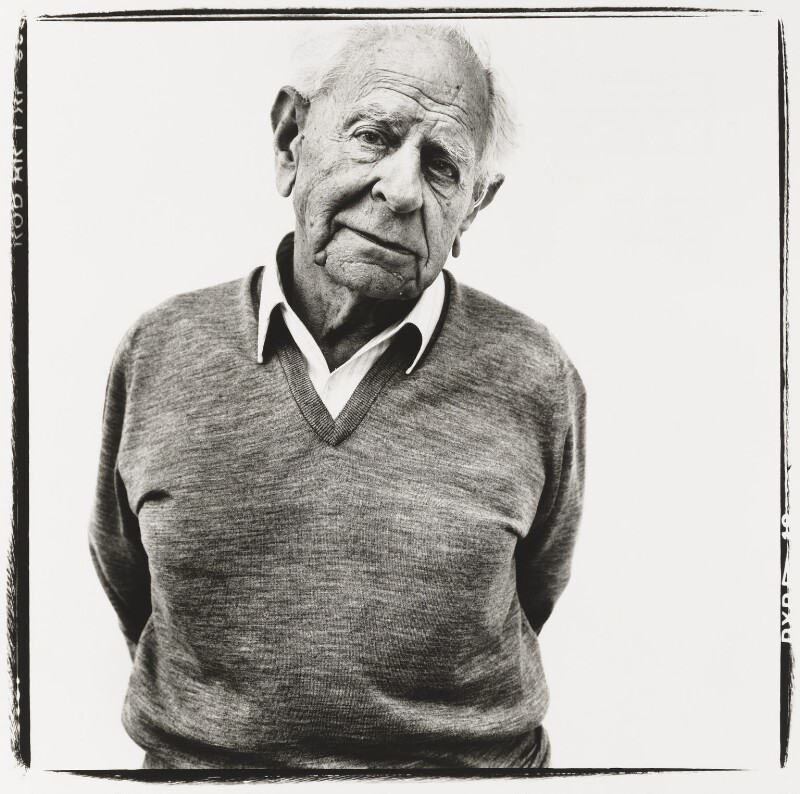
\includegraphics[width=0.5\textwidth,height=\textheight]{images/karl-popper.png}

\legend{Source:
\href{https://www.npg.org.uk/collections/search/portrait/mw08238/Sir-Karl-Raimund-Popper?}{Steve
Pyke}.}

}

\end{figure}%

\section{Secondary section}\label{secondary-section}

See Table~\ref{tbl-iris}.

\index{tables}

\begin{Shaded}
\begin{Highlighting}[numbers=left,,]
\NormalTok{datasets}\SpecialCharTok{::}\NormalTok{iris }\SpecialCharTok{|\textgreater{}}
\NormalTok{  dplyr}\SpecialCharTok{::}\FunctionTok{as\_tibble}\NormalTok{() }\SpecialCharTok{|\textgreater{}}
\NormalTok{  dplyr}\SpecialCharTok{::}\FunctionTok{slice\_sample}\NormalTok{(}\AttributeTok{n =} \DecValTok{5}\NormalTok{) }\SpecialCharTok{|\textgreater{}}
\NormalTok{  gt}\SpecialCharTok{::}\FunctionTok{gt}\NormalTok{()}
\end{Highlighting}
\end{Shaded}

\begin{table}

\caption{\label{tbl-iris}A sample of the famous (Fisher's or Anderson's)
iris data set}

\centering{

\begin{longtable*}{rrrrc}
\toprule
Sepal.Length & Sepal.Width & Petal.Length & Petal.Width & Species \\ 
\midrule\addlinespace[2.5pt]
6.5 & 3.0 & 5.5 & 1.8 & virginica \\ 
6.5 & 3.0 & 5.8 & 2.2 & virginica \\ 
5.0 & 3.0 & 1.6 & 0.2 & setosa \\ 
5.0 & 3.5 & 1.6 & 0.6 & setosa \\ 
6.2 & 2.9 & 4.3 & 1.3 & versicolor \\ 
\bottomrule
\end{longtable*}

\legend{Source: Based on \textcite{fisher1936}.}

}

\end{table}%

\subsection{Tertiary section}\label{tertiary-section}

\index{figures!chart}

\begin{Shaded}
\begin{Highlighting}[numbers=left,,]
\NormalTok{ggplot2}\SpecialCharTok{::}\FunctionTok{ggplot}\NormalTok{(}
  \AttributeTok{data =}\NormalTok{ datasets}\SpecialCharTok{::}\NormalTok{faithful, }
  \AttributeTok{mapping =}\NormalTok{ ggplot2}\SpecialCharTok{::}\FunctionTok{aes}\NormalTok{(}\AttributeTok{x =}\NormalTok{ eruptions, }\AttributeTok{y =}\NormalTok{ waiting)}
\NormalTok{  ) }\SpecialCharTok{+}
\NormalTok{  ggplot2}\SpecialCharTok{::}\FunctionTok{geom\_point}\NormalTok{() }\SpecialCharTok{+}
\NormalTok{  ggplot2}\SpecialCharTok{::}\FunctionTok{xlim}\NormalTok{(}\FloatTok{0.5}\NormalTok{, }\DecValTok{6}\NormalTok{) }\SpecialCharTok{+}
\NormalTok{  ggplot2}\SpecialCharTok{::}\FunctionTok{ylim}\NormalTok{(}\DecValTok{40}\NormalTok{, }\DecValTok{110}\NormalTok{) }\SpecialCharTok{+}
\NormalTok{  ggplot2}\SpecialCharTok{::}\FunctionTok{geom\_density\_2d\_filled}\NormalTok{(}\AttributeTok{alpha =} \FloatTok{0.5}\NormalTok{) }\SpecialCharTok{+}
\NormalTok{  ggplot2}\SpecialCharTok{::}\FunctionTok{geom\_density\_2d}\NormalTok{(}\AttributeTok{linewidth =} \FloatTok{0.25}\NormalTok{, }\AttributeTok{colour =} \StringTok{"black"}\NormalTok{) }\SpecialCharTok{+}
\NormalTok{  ggplot2}\SpecialCharTok{::}\FunctionTok{theme}\NormalTok{(}\AttributeTok{legend.position =} \StringTok{"none"}\NormalTok{)}
\end{Highlighting}
\end{Shaded}

\begin{figure}[H]

\caption{\label{fig-eruption}Relationship between \emph{waiting time to
next eruption} (minutes) and \emph{eruption time} (minutes) at Old
Faithful Geyser, Yellowstone National Park, Wyoming, USA}

\centering{

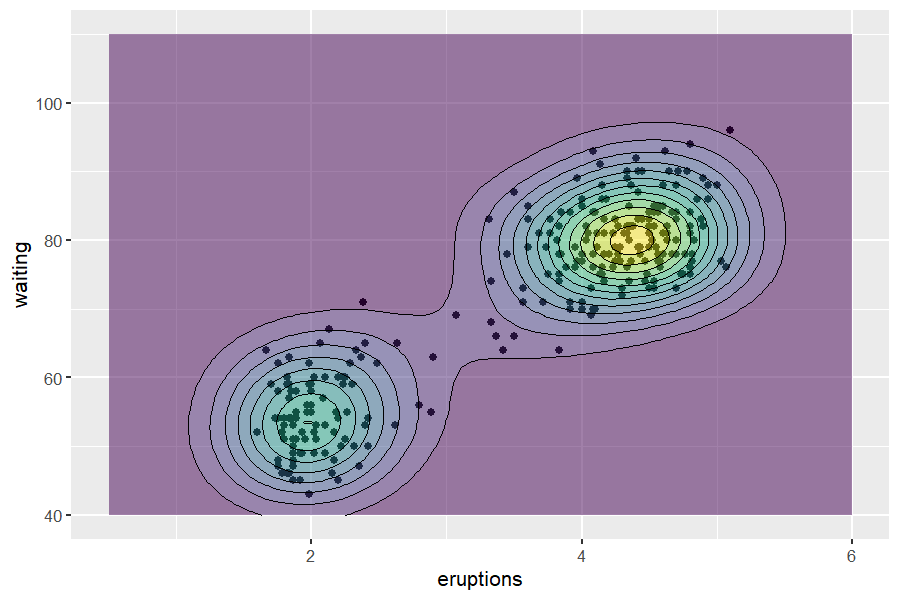
\includegraphics{index_files/figure-pdf/unnamed-chunk-5-1.png}

\legend{Source: Retrieved from the
\href{https://ggplot2.tidyverse.org/reference/geom_density_2d.html}{\texttt{ggplot2}
R package documentation} \autocite{wickham2016a}.}

}

\end{figure}%

\clearpage

\subsubsection{Quaternary section}\label{quaternary-section}

\begin{itemize}
\tightlist
\item
  Bullet point

  \begin{itemize}
  \tightlist
  \item
    Bullet point

    \begin{itemize}
    \tightlist
    \item
      Bullet point
    \end{itemize}
  \end{itemize}
\end{itemize}

\paragraph{Quinary section}\label{quinary-section}

\begin{enumerate}
\def\labelenumi{\arabic{enumi}.}
\tightlist
\item
  List
\item
  List
\item
  List
\end{enumerate}

\section{Another secondary section}\label{another-secondary-section}

See Figure~\ref{fig-mpg}.

\index{figures!chart}

\begin{Shaded}
\begin{Highlighting}[numbers=left,,]
\NormalTok{p }\OtherTok{\textless{}{-}}\NormalTok{ ggplot2}\SpecialCharTok{::}\FunctionTok{ggplot}\NormalTok{(}
  \AttributeTok{data =}\NormalTok{ datasets}\SpecialCharTok{::}\NormalTok{mtcars, }
  \AttributeTok{mapping =}\NormalTok{ ggplot2}\SpecialCharTok{::}\FunctionTok{aes}\NormalTok{(}\AttributeTok{x=}\NormalTok{wt, }\AttributeTok{y=}\NormalTok{mpg, }\AttributeTok{color=}\NormalTok{cyl, }\AttributeTok{size=}\NormalTok{cyl)}
\NormalTok{  ) }\SpecialCharTok{+}
\NormalTok{  ggplot2}\SpecialCharTok{::}\FunctionTok{geom\_point}\NormalTok{() }\SpecialCharTok{+}
\NormalTok{  ggplot2}\SpecialCharTok{::}\FunctionTok{theme}\NormalTok{(}\AttributeTok{legend.position=}\StringTok{"none"}\NormalTok{)}

\NormalTok{ggExtra}\SpecialCharTok{::}\FunctionTok{ggMarginal}\NormalTok{(}
  \AttributeTok{p =}\NormalTok{ p, }
  \AttributeTok{type =} \StringTok{"histogram"}\NormalTok{, }
  \AttributeTok{fill =} \StringTok{"slateblue"}\NormalTok{, }
  \AttributeTok{xparams =} \FunctionTok{list}\NormalTok{(}\AttributeTok{bins=}\DecValTok{10}\NormalTok{)}
\NormalTok{)}
\end{Highlighting}
\end{Shaded}

\begin{figure}[H]

\caption{\label{fig-mpg}Relation between \emph{weight (1000lbs)}
(\(\text{wt}\)) and \emph{miles per galon} (\(\text{mpg}\)) for
combustion engine vehicles}

\centering{

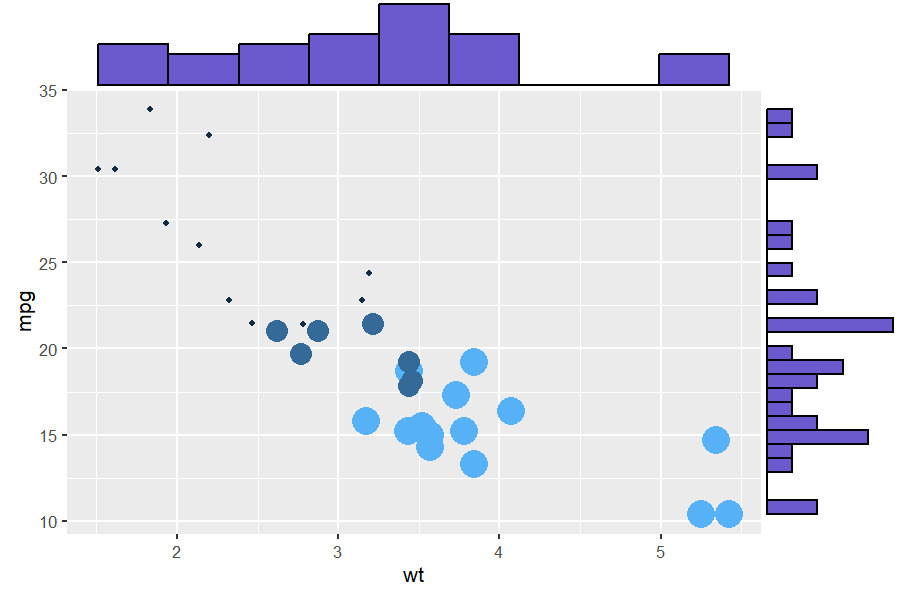
\includegraphics{index_files/figure-pdf/unnamed-chunk-6-1.png}

\legend{Source: Data extracted from the 1974 Motor Trend magazine and
published by \textcite{henderson1981}. Visualization by
\textcite{holtz}, available at
\href{https://r-graph-gallery.com/277-marginal-histogram-for-ggplot2.html}{The
R Graph Gallery}.}

}

\end{figure}%

\bookmarksetup{startatroot}

\chapter{{[}Showcase{]} Development}\label{sec-development}

\begin{tcolorbox}[enhanced jigsaw, toptitle=1mm, colbacktitle=quarto-callout-warning-color!10!white, rightrule=.15mm, colframe=quarto-callout-warning-color-frame, leftrule=.75mm, opacityback=0, breakable, bottomtitle=1mm, arc=.35mm, coltitle=black, colback=white, title=\textcolor{quarto-callout-warning-color}{\faExclamationTriangle}\hspace{0.5em}{Warning}, opacitybacktitle=0.6, titlerule=0mm, bottomrule=.15mm, left=2mm, toprule=.15mm]

The text below is for demonstrative purposes only.

\vspace{0.25\baselineskip}

See \url{https://github.com/danielvartan/abnt} to learn more about this
template.

\end{tcolorbox}

Cillum qui eu non ipsum pariatur ad exercitation pariatur dolore veniam
amet cillum. Aliqua do nostrud aliquip in amet. Commodo sit tempor nulla
ipsum officia voluptate laborum elit minim proident Lorem. Id pariatur
reprehenderit non officia fugiat incididunt anim aliquip anim anim.
Ipsum irure magna quis est aute. Nostrud nulla mollit non labore. In
laboris mollit ea in. Excepteur eu do elit proident. Commodo tempor nisi
enim ex velit voluptate dolor mollit eiusmod in ullamco aliqua nostrud
id.

Eiusmod dolore sint proident consectetur reprehenderit exercitation
sunt. Nisi qui sit commodo anim consectetur in laborum dolore in labore
veniam labore commodo tempor. Sunt sit officia commodo quis magna.
Aliqua esse est adipisicing ea est ex esse esse officia sit culpa minim
amet dolore. Culpa dolore laborum sunt do commodo duis in velit. Mollit
duis voluptate aliquip magna labore aute sit dolore amet culpa labore.
Id tempor consectetur est anim ullamco ex nostrud voluptate excepteur.
Aliqua laboris aute laborum amet eu. Minim quis veniam et dolor quis
fugiat. Adipisicing amet est do aliqua nostrud amet excepteur ut.

\section{Secondary section}\label{secondary-section-1}

Minim consectetur eu aliqua in elit incididunt labore amet consequat
cillum minim. Id sit duis duis ex velit proident mollit minim consequat
nulla. Aliqua elit do excepteur nulla nostrud exercitation nisi tempor
incididunt. Veniam dolore in non nisi veniam aliquip. Minim labore
excepteur ea est dolore laboris cillum. Laboris sit pariatur pariatur
veniam mollit nisi cupidatat qui qui quis laborum veniam dolor. Proident
aliquip do adipisicing dolor elit aute elit. Officia anim quis id
voluptate eu. Quis labore consectetur est magna. Laborum nulla ea non
Lorem officia aute.

\bookmarksetup{startatroot}

\chapter{{[}Showcase{]} Conclusion}\label{sec-conclusion}

\begin{tcolorbox}[enhanced jigsaw, toptitle=1mm, colbacktitle=quarto-callout-important-color!10!white, rightrule=.15mm, colframe=quarto-callout-important-color-frame, leftrule=.75mm, opacityback=0, breakable, bottomtitle=1mm, arc=.35mm, coltitle=black, colback=white, title=\textcolor{quarto-callout-important-color}{\faExclamation}\hspace{0.5em}{Important}, opacitybacktitle=0.6, titlerule=0mm, bottomrule=.15mm, left=2mm, toprule=.15mm]

The text below is for demonstrative purposes only.

\vspace{0.25\baselineskip}

See \url{https://github.com/danielvartan/abnt} to learn more about this
template.

\end{tcolorbox}

Cillum qui eu non ipsum pariatur ad exercitation pariatur dolore veniam
amet cillum. Aliqua do nostrud aliquip in amet. Commodo sit tempor nulla
ipsum officia voluptate laborum elit minim proident Lorem. Id pariatur
reprehenderit non officia fugiat incididunt anim aliquip anim anim.
Ipsum irure magna quis est aute. Nostrud nulla mollit non labore. In
laboris mollit ea in. Excepteur eu do elit proident. Commodo tempor nisi
enim ex velit voluptate dolor mollit eiusmod in ullamco aliqua nostrud
id.

Eiusmod dolore sint proident consectetur reprehenderit exercitation
sunt. Nisi qui sit commodo anim consectetur in laborum dolore in labore
veniam labore commodo tempor. Sunt sit officia commodo quis magna.
Aliqua esse est adipisicing ea est ex esse esse officia sit culpa minim
amet dolore. Culpa dolore laborum sunt do commodo duis in velit. Mollit
duis voluptate aliquip magna labore aute sit dolore amet culpa labore.
Id tempor consectetur est anim ullamco ex nostrud voluptate excepteur.
Aliqua laboris aute laborum amet eu. Minim quis veniam et dolor quis
fugiat. Adipisicing amet est do aliqua nostrud amet excepteur ut.

\section{Secondary section}\label{secondary-section-2}

Minim consectetur eu aliqua in elit incididunt labore amet consequat
cillum minim. Id sit duis duis ex velit proident mollit minim consequat
nulla. Aliqua elit do excepteur nulla nostrud exercitation nisi tempor
incididunt. Veniam dolore in non nisi veniam aliquip. Minim labore
excepteur ea est dolore laboris cillum. Laboris sit pariatur pariatur
veniam mollit nisi cupidatat qui qui quis laborum veniam dolor. Proident
aliquip do adipisicing dolor elit aute elit. Officia anim quis id
voluptate eu. Quis labore consectetur est magna. Laborum nulla ea non
Lorem officia aute.

\postextual

\begingroup
\renewcommand{\baselinestretch}{1}
\setcounter{footnote}{0}
\renewcommand{\thefootnote}{\fnsymbol{footnote}}
\printbibliography[heading=bibheading]
\endgroup

\tocskipone
\tocprintchapternonum
\addcontentsline{toc}{chapter}{\newbibname}

\begin{glossario}

\bookmarksetup{startatroot}

\chapter*{Glossary}\label{glossary}
\addcontentsline{toc}{chapter}{Glossary}

\markboth{Glossary}{Glossary}

For an extensive list of chronobiology related terms and definitions,
please refer to \textcite{aschoff1965} and \textcite{marques2012}.

\begin{description}
\item[Chronotype]
\hspace{20cm}

Any kind of temporal phenotype \autocite{ehret1974,pittendrigh1993}.
Usually, it refers to circadian phenotypes in a spectrum that goes from
morningness to eveningness \autocite{roenneberg2003}. It can also be
seen as an organism's phase of entrainment \autocite{roenneberg2012a}.
\item[Circadian rhythm]
\hspace{20cm}

A rhythm with a period close to a day/24h, an approximation to the
period of the earth's rotation \autocite{pittendrigh1960}. From the
Latin \emph{circā}, around, and \emph{dĭes}, day \autocite{latinitium}.
Example: the sleep-wake cycle.
\item[Complex system]
\hspace{20cm}

There are several definitions. Here are some that I found to be of use:
\end{description}

\begin{itemize}
\tightlist
\item
  ``Systems that don't yield to compact forms of representation or
  description'' (David Krakauer apud \textcite{mitchell2013})
\item
  ``A system of many interacting parts where the system is more than
  just the sum of its parts'' (Mark Newman apud \textcite{mitchell2013})
\item
  Systems with many connected agents that interact and exhibit
  self-organization and emergence behavior, all without the need for a
  central controller (adapted from Camilo Rodrigues Neto's definition,
  supervisor of this thesis).
\item
  Dialectics at its finest (my working definition).
\end{itemize}

\begin{description}
\item[Entrainment]
\hspace{20cm}

A shift and alignment of biological rhythms induced by a zeitgeber input
\autocite{kuhlman2018}. For example: a shift/alignment of an organism's
circadian rhythm when exposed to light.
\end{description}

\end{glossario}

\begin{apendicesenv}

\cleardoublepage
\phantomsection
\addcontentsline{toc}{part}{Appendices}
\appendix

\chapter{{[}Showcase{]}}\label{sec-appendix-a}

\begin{tcolorbox}[enhanced jigsaw, toptitle=1mm, colbacktitle=quarto-callout-tip-color!10!white, rightrule=.15mm, colframe=quarto-callout-tip-color-frame, leftrule=.75mm, opacityback=0, breakable, bottomtitle=1mm, arc=.35mm, coltitle=black, colback=white, title=\textcolor{quarto-callout-tip-color}{\faLightbulb}\hspace{0.5em}{Tip}, opacitybacktitle=0.6, titlerule=0mm, bottomrule=.15mm, left=2mm, toprule=.15mm]

The text below is for demonstrative purposes only.

\vspace{0.25\baselineskip}

See \url{https://quarto.org/docs/authoring/markdown-basics.html} to
learn about the basics of Markdown's syntax.

\end{tcolorbox}

Cillum qui eu non ipsum pariatur ad exercitation pariatur dolore veniam
amet cillum. Aliqua do nostrud aliquip in amet. Commodo sit tempor nulla
ipsum officia voluptate laborum elit minim proident Lorem. Id pariatur
reprehenderit non officia fugiat incididunt anim aliquip anim anim.
Ipsum irure magna quis est aute. Nostrud nulla mollit non labore. In
laboris mollit ea in. Excepteur eu do elit proident. Commodo tempor nisi
enim ex velit voluptate dolor mollit eiusmod in ullamco aliqua nostrud
id.

Eiusmod dolore sint proident consectetur reprehenderit exercitation
sunt. Nisi qui sit commodo anim consectetur in laborum dolore in labore
veniam labore commodo tempor. Sunt sit officia commodo quis magna.
Aliqua esse est adipisicing ea est ex esse esse officia sit culpa minim
amet dolore. Culpa dolore laborum sunt do commodo duis in velit. Mollit
duis voluptate aliquip magna labore aute sit dolore amet culpa labore.
Id tempor consectetur est anim ullamco ex nostrud voluptate excepteur.
Aliqua laboris aute laborum amet eu. Minim quis veniam et dolor quis
fugiat. Adipisicing amet est do aliqua nostrud amet excepteur ut.

\section{Secondary section}\label{secondary-section-3}

Minim consectetur eu aliqua in elit incididunt labore amet consequat
cillum minim. Id sit duis duis ex velit proident mollit minim consequat
nulla. Aliqua elit do excepteur nulla nostrud exercitation nisi tempor
incididunt. Veniam dolore in non nisi veniam aliquip. Minim labore
excepteur ea est dolore laboris cillum. Laboris sit pariatur pariatur
veniam mollit nisi cupidatat qui qui quis laborum veniam dolor. Proident
aliquip do adipisicing dolor elit aute elit. Officia anim quis id
voluptate eu. Quis labore consectetur est magna. Laborum nulla ea non
Lorem officia aute.

\chapter{PDF Settings}\label{sec-settings}

\begin{tcolorbox}[enhanced jigsaw, toptitle=1mm, colbacktitle=quarto-callout-important-color!10!white, rightrule=.15mm, colframe=quarto-callout-important-color-frame, leftrule=.75mm, opacityback=0, breakable, bottomtitle=1mm, arc=.35mm, coltitle=black, colback=white, title=\textcolor{quarto-callout-important-color}{\faExclamation}\hspace{0.5em}{Important}, opacitybacktitle=0.6, titlerule=0mm, bottomrule=.15mm, left=2mm, toprule=.15mm]

You are reading the work-in-progress of this manual.

\vspace{0.25\baselineskip}

This chapter is undergoing heavy restructuring and may be confusing or
incomplete.

\end{tcolorbox}

\section{Typography}\label{typography}

\index{tipography}

\subsection{Typeface}\label{typeface}

To change typefaces, simply use the
\href{https://quarto.org/docs/reference/formats/pdf.html}{Quarto
options}, such as \texttt{mainfont}, \texttt{monofont} and
\texttt{sansfont} in your \texttt{quarto-{[}format{]}.yml} file.

\begin{Shaded}
\begin{Highlighting}[numbers=left,,]
\FunctionTok{format}\KeywordTok{:}
\AttributeTok{  }\FunctionTok{abnt{-}pdf}\KeywordTok{:}
\AttributeTok{    }\FunctionTok{mainfont}\KeywordTok{:}\AttributeTok{ Arial}
\end{Highlighting}
\end{Shaded}

The ABNT NBR 14724:2011 norm does not specify the use of any specific
font. You have the freedom to choose any font you prefer, but it's
important to note that the selected font must be installed on your
computer.

\subsection{Font size}\label{font-size}

To adjust the font size, utilize the \texttt{fontsize} option in in the
\texttt{quarto-{[}format{]}.yml} file.

\begin{Shaded}
\begin{Highlighting}[numbers=left,,]
\FunctionTok{format}\KeywordTok{:}
\AttributeTok{  }\FunctionTok{abnt{-}pdf}\KeywordTok{:}
\AttributeTok{    }\FunctionTok{fontsize}\KeywordTok{:}\AttributeTok{ 12pt}
\end{Highlighting}
\end{Shaded}

It's important to note that the third paragraph of Section 5.1 of ABNT
NBR 14724:2011 norm establishes that the font size should be 12pt for
the entire document, including the cover, except for quotations longer
than three lines, footnotes, pagination, cataloging data, captions, and
sources of illustrations and tables, which should be in a smaller and
uniform size.

The smaller font is set to \texttt{\textbackslash{}footnotesize}, which
corresponds to a 10pt font size with the default settings. You can
modify this setting by inserting the following LaTeX command into
\texttt{tex/include-in-header.tex}:

\begin{Shaded}
\begin{Highlighting}[numbers=left,,]
\FunctionTok{\textbackslash{}renewcommand}\NormalTok{\{}\ExtensionTok{\textbackslash{}ABNTEXfontereduzida}\NormalTok{\}\{[NEW SIZE (e.g., }\FunctionTok{\textbackslash{}small}\NormalTok{)]\}}
\end{Highlighting}
\end{Shaded}

\section{Language and hyphenation}\label{language-and-hyphenation}

\section{Document sections}\label{document-sections}

\subsection{Editing pre-textual
sections}\label{editing-pre-textual-sections}

\texttt{abnt} uses a system of tags to transfer and render the content
of Quarto files (\texttt{.qmd}) to LaTeX. These tags look like this:

\begin{Shaded}
\begin{Highlighting}[numbers=left,,]
\CommentTok{\%:::\% class attribute begin/end \%:::\%}
\end{Highlighting}
\end{Shaded}

\begin{Shaded}
\begin{Highlighting}[numbers=left,,]
\CommentTok{\textless{}!{-}{-} \%:::\% class attribute begin/end \%:::\% {-}{-}\textgreater{}}
\end{Highlighting}
\end{Shaded}

Unless you want to customize the template, you don't need to modify the
\texttt{.tex} files. You can write directly in the \texttt{.qmd} files.
Just ensure that you preserve all the tags.

Please note that some settings regarding the pre-textual sections must
be changed in the \texttt{qmd/\_congfig.qmd} file.

\subsection{\texorpdfstring{How to include LaTeX commands in Quarto
files
(\texttt{.qmd})}{How to include LaTeX commands in Quarto files (.qmd)}}\label{how-to-include-latex-commands-in-quarto-files-.qmd}

To add LaTeX commands in your writing, without worrying that it will
contaminate the \texttt{html} format, use a \texttt{\{=latex\}} chunk.

\begin{Shaded}
\begin{Highlighting}[numbers=left,,]
\NormalTok{\textasciigrave{}\textasciigrave{}\textasciigrave{}\{=latex\}}
\CommentTok{\% Some LaTeX code.}
\NormalTok{\textasciigrave{}\textasciigrave{}\textasciigrave{}}
\end{Highlighting}
\end{Shaded}

\subsection{How to add or remove
sections}\label{how-to-add-or-remove-sections}

For pre-textual sections (e.g., list of symbols, abstract), remove them
from \texttt{tex/include-before-body.tex} and from
\texttt{R/quarto-pre-render.R}.

For textual sections (e.g., chapters), remove them from
\texttt{.quarto-{[}format{]}.yml} file.

For post-textual sections (e.g., appendices, annexes):

\begin{itemize}
\tightlist
\item
  If it's the Glossary, remove it from \texttt{.quarto-{[}format{]}.yml}
  and copy the the LaTeX code after
  \texttt{\textless{}!-\/-\ glossary\ end\ -\/-\textgreater{}} in
  \texttt{glossary.qmd} to the bottom of the last chapter;
\item
  If it's not the last appendix chapter, simply remove it from
  \texttt{.quarto-{[}format{]}.yml}; else remove it from
  \texttt{.quarto-{[}format{]}.yml}, remove
  \texttt{\textbackslash{}begin\{apendicesenv\}} from the bottom of
  \texttt{glossary.qmd} and add the code the code after
  \texttt{\textless{}!-\/-\ appendices\ end\ -\/-\textgreater{}} of the
  appendice file to the bottom of \texttt{glossary.qmd};
\item
  {[}Annexes{]};
\item
  {[}Index{]}.
\end{itemize}

It's important to note that, at this moment, the transition between
sections of the document are made inserting LaTeX code at the end of
specific sections. These are:

\begin{itemize}
\tightlist
\item
  Between the last chapter and the Glossary section.
\item
  Between the Glossary section and the Appendices section.
\item
  Between the Appendices and Annexes section.
\item
  After the Annexes section.
\end{itemize}

\section{Citation management}\label{citation-management}

\subsection{Citation method}\label{citation-method}

\index{BibLaTeX}

This Quarto format was specifically designed to be compatible with
\href{https://www.ctan.org/pkg/biblatex}{BibLaTeX}, which is a
comprehensive reimplementation of
\href{https://www.bibtex.org/}{BiBTeX}. At first glance, these two
systems may appear very similar.

To get started, simply insert your references into the
\texttt{references.bib}file. However, this task can be somewhat tedious
and demanding. To simplify the process, we recommend exploring the
integration of \href{https://www.zotero.org/}{Zotero} along with
\href{https://github.com/retorquere/zotero-better-bibtex}{Better
BiBTeX}, as demonstrated in a section below.

For detailed guidance on handling citations in Quarto, please refer to
Quarto's
\href{https://quarto.org/docs/authoring/footnotes-and-citations.html}{Citation
\& Footnotes} documentation.

\subsection{Citation style}\label{citation-style}

\index{ABNT}
\index{APA}

There are two built-in citation styles:

\begin{itemize}
\tightlist
\item
  \href{https://www.abnt.org.br/}{ABNT} (Brazilian Association of
  Technical Standards);
\item
  \href{https://apastyle.apa.org/}{APA} (American Psychological
  Association).
\end{itemize}

To use one of them, simply change the \texttt{biblio-style} option in
your \texttt{yml} file with the style of you preference.

\begin{Shaded}
\begin{Highlighting}[numbers=left,,]
\FunctionTok{format}\KeywordTok{:}
\AttributeTok{  }\FunctionTok{abnt{-}pdf}\KeywordTok{:}
\AttributeTok{    }\FunctionTok{biblio{-}style}\KeywordTok{:}\AttributeTok{ abnt}\CommentTok{ \# options: [abnt, abnt{-}ibid, abnt{-}numeric, apa]}
\end{Highlighting}
\end{Shaded}

There are other options related to the citation style; some are shown
below. Please refer to
\href{https://www.ctan.org/pkg/biblatex}{\texttt{biblatex}},
\href{https://www.ctan.org/pkg/biblatex-abnt}{\texttt{biblatex-abnt}}
and \href{https://www.ctan.org/pkg/biblatex-apa}{\texttt{biblatex-apa}}
manuals to learn more about them.

\begin{Shaded}
\begin{Highlighting}[numbers=left,,]
\FunctionTok{format}\KeywordTok{:}
\AttributeTok{  }\FunctionTok{abnt{-}pdf}\KeywordTok{:}
\FunctionTok{    biblio{-}footnote}\KeywordTok{: }\CharTok{\textgreater{}}
\NormalTok{      According to the Brazilian Association of Technical Standards}
\NormalTok{      (ABNT NBR 6023).}
\AttributeTok{    }\FunctionTok{biblatexoptions}\KeywordTok{:}
\AttributeTok{      }\KeywordTok{{-}}\AttributeTok{ backend=biber,}
\AttributeTok{      }\KeywordTok{{-}}\AttributeTok{ language=english,}\CommentTok{ \# [options: english, brazil, spanish, french]}
\AttributeTok{      }\KeywordTok{{-}}\AttributeTok{ url=true,}
\AttributeTok{      }\KeywordTok{{-}}\AttributeTok{ useprefix=false,}
\AttributeTok{      }\KeywordTok{{-}}\AttributeTok{ giveninits=true,}
\AttributeTok{      }\KeywordTok{{-}}\AttributeTok{ extrayear=true}
\AttributeTok{    }\FunctionTok{bibhang}\KeywordTok{:}\AttributeTok{ 0cm}\CommentTok{ \# Use 0.5cm if \textasciigrave{}biblio{-}style: apa\textasciigrave{}.}
\AttributeTok{    }\FunctionTok{bibparsep}\KeywordTok{:}\AttributeTok{ 0ex}
\end{Highlighting}
\end{Shaded}

\subsection{Zotero integration}\label{zotero-integration}

\index{Zotero}
\index{Better BiBTeX}

This template can work with \href{https://www.zotero.org/}{Zotero} and
the \href{https://github.com/retorquere/zotero-better-bibtex}{Better
BiBTeX} plugin. The advantage of using this integration is that you
don't need to manually input your references into
\texttt{references.bib}; they are automatically imported when you render
the format.

For this to work, you must activate the \texttt{zotero} option in your
\texttt{yml} file and have Zotero, with Better BibTeX installed, open
while rendering your thesis (activated by default). A pre-render script
(see \texttt{R/quarto-pre-render.R}), created using the
\href{https://github.com/paleolimbot/rbbt}{\texttt{rbbt}} R package,
will scan all \texttt{.qmd} and \texttt{.tex} files searching for BibTeX
citations (e.g., \texttt{@watson1953}). If they match with your Zotero
database, the citations will then be written into the
\texttt{references.bib} file.

\begin{Shaded}
\begin{Highlighting}[numbers=left,,]
\FunctionTok{format}\KeywordTok{:}
\AttributeTok{  }\FunctionTok{abnt{-}pdf}\KeywordTok{:}
\AttributeTok{    }\FunctionTok{zotero}\KeywordTok{:}\AttributeTok{ }\CharTok{true}
\end{Highlighting}
\end{Shaded}

\subsubsection{Title case change}\label{title-case-change}

\index{BibLaTeX}

By using \href{https://www.zotero.org/}{Zotero}, you may experience a
title casing change when exporting your references. This is the default
behavior of \href{https://retorque.re/zotero-better-bibtex/}{Better
BibTex} while exporting to BibLaTeX.

You can disable this by going to Zotero's configuration editor (go to
Edit \textgreater{} Preferences \textgreater{} Advanced \textgreater{}
Config Editor) and changing the variable\textbackslash{}
\texttt{extensions.zotero.translators.better-bibtex.exportTitleCase} to
\texttt{false}. Beware that this can produce some issues. You can find
more information about this behavior
\href{https://retorque.re/zotero-better-bibtex/support/faq/\#bbt-is-changing-the-capitalization-of-my-titles----why}{here}.

\section{ABNT figures and tables}\label{abnt-figures-and-tables}

Thanks for the incredible work of
\href{https://github.com/cscheid}{Carlos Scheidegger} and other Quarto
developers we now have a built-in solution for figures and tables that
require two captions (one at the top and the other at the bottom, or a
caption and a legend), as required by the ABNT norms. Please note that
this feature is only available for Quarto versions \textgreater=v1.4.

The procedure for adding these captions is the same for figures and
tables. Enclose your figure/table/code in figure \texttt{divs}, as shown
in the example below. The first paragraph after the figure content will
be rendered as the source (bottom caption), and the last one will be the
top caption.

The formatting options for this bottom caption/legend is still matter of
debate (see
\href{https://github.com/quarto-dev/quarto-cli/discussions/6103\#discussioncomment-7494661}{here}).
That's why is important to add Quarto's
\href{https://github.com/quarto-ext/latex-environment}{LaTeX
Environment} filter in your
\texttt{\_quarto-pdf.yml"\ with\ the\ command}legend\texttt{and\ use}{[}SOURCE
TEXT GOES HERE{]}.legend\}` when defining legends for figures/tables,
like the example below.

\begin{Shaded}
\begin{Highlighting}[numbers=left,,]
\NormalTok{::: \{\#fig{-}1\}}

\NormalTok{::: \{.figure{-}content\}}
\NormalTok{This is the figure content.}
\NormalTok{:::}

\CommentTok{[}\OtherTok{Source: My source.}\CommentTok{]}\NormalTok{\{.legend\}}

\NormalTok{This is a caption.}

\NormalTok{:::}
\end{Highlighting}
\end{Shaded}

Please note that, like all cross-reference elements, these \texttt{divs}
must follow a naming pattern. Always use the prefixes \texttt{\#fig-}
for figures and \texttt{\#tbl-} for tables.

Visit the showcase chapter ``Introduction''
(\texttt{qmd/introduction.qmd}) of this Quarto format to see this
feature in action. For more detailed information, please refer to
Quarto's
\href{https://quarto.org/docs/prerelease/1.4/crossref.html}{Crossreferenceable
elements} article.

\section{Redenring PDF after rendering HTML (and
vice-versa)}\label{redenring-pdf-after-rendering-html-and-vice-versa}

The index file title (\texttt{index.qmd}) and content must be altered
for each format to render properly. This cause some issues that
\texttt{abnt} can't resolve for now. If you've rendered the HTML format
and them wish to render the PDF format, you must run
\texttt{R/quarto-pre-render-pdf.R} one time before starting the render.
If is the inverse situation, you must run one time
\texttt{R/quarto-pre-render-html.R}.

We're working to fix this.

\section{Crossreferenceable elements}\label{crossreferenceable-elements}

Quarto allow you to create and reference almost anything by using div
enclosures.

Example: See Theorem~\ref{thm-line}.

\begin{theorem}[Line]\protect\hypertarget{thm-line}{}\label{thm-line}

The equation of any straight line, called a linear equation, can be
written as:

\[
y = mx + b
\]

\end{theorem}

Although, it's important to note that for this to work, each type of
\texttt{div} must use pre-defined prefixes. If you don't follow these
rules your document will not be rendered.

Here are most of the the label prefixes.

\begin{figure}

\begin{minipage}[t]{0.33\linewidth}

\begin{itemize}
\tightlist
\item
  \texttt{cnj-}: Conjecture
\item
  \texttt{cor-}: Corollary
\item
  \texttt{def-}: Definition
\item
  \texttt{eq-}: Equation
\item
  \texttt{exm-}: Example
\end{itemize}

\end{minipage}%
%
\begin{minipage}[t]{0.33\linewidth}

\begin{itemize}
\tightlist
\item
  \texttt{exr-}: Exercise
\item
  \texttt{fig-}: Figure
\item
  \texttt{lem-}: Lemma
\item
  \texttt{lst-}: Listings
\end{itemize}

\end{minipage}%
%
\begin{minipage}[t]{0.33\linewidth}

\begin{itemize}
\tightlist
\item
  \texttt{prp-}: Proposition
\item
  \texttt{sec-}: Section
\item
  \texttt{tbl-}: Table
\item
  \texttt{thm-}: Theorem
\end{itemize}

\end{minipage}%

\end{figure}%

For more information about cross-reference elements, see Quarto's
guide\href{https://quarto.org/docs/books/book-crossrefs.html}{Book
Crossrefs},
\href{https://quarto.org/docs/authoring/cross-references.html}{Cross
References} and
\href{https://quarto.org/docs/prerelease/1.4/crossref.html}{Crossreferenceable
elements} articles.

\section{Freezing and cache}\label{freezing-and-cache}

See
\href{https://quarto.org/docs/projects/code-execution.html\#freeze}{Freeze}.

\section{How to customize this Quarto
format}\label{how-to-customize-this-quarto-format}

\subsection{Quarto system}\label{quarto-system}

See \href{https://quarto.org/docs/guide/}{Quarto's guide}.

\subsection{Template and template
partials}\label{template-and-template-partials}

See
\href{https://quarto.org/docs/journals/templates.html\#template-partials}{Tempalte
partials}.

\subsection{Spacing rules}\label{spacing-rules}

\begin{itemize}
\tightlist
\item
  Set fixed dimensions (e.g., page dimensions) in \texttt{cm} or
  \texttt{pt}. \texttt{cm} is the prefer unit for margins.
\item
  Set line spacing as a proportion of
  \texttt{\textbackslash{}baselineskip} (e.g.,
  \texttt{1.5\textbackslash{}baselineskip}).
\item
  Use the settings \texttt{\textbackslash{}tinyskipamount},
  \texttt{\textbackslash{}smallskipamount},
  \texttt{\textbackslash{}midskipamount},
  \texttt{\textbackslash{}bigskipamount},
  \texttt{\textbackslash{}hugeskipamount} and their counterparts
  \texttt{\textbackslash{}tinyskip}, \texttt{\textbackslash{}smallskip},
  \texttt{\textbackslash{}midskip}, \texttt{\textbackslash{}bigskip},
  \texttt{\textbackslash{}hugeskip}. You can find them in the
  \texttt{lengths.tex} template partial.
\item
  For other kinds of relative vertical spacing, use the \texttt{ex}
  unit.
\item
  For relative horizontal spacing, use the \texttt{em} unit.
\end{itemize}

See \textcite[section 7.5]{oetiker2023} to learn more about LaTeX
spacing features. The articles on
\href{https://www.overleaf.com}{Overleaf} are also a great source of
information. Check
\href{https://www.overleaf.com/learn/latex/Lengths_in_LaTeX}{Lengths in
LaTeX} and
\href{https://www.overleaf.com/learn/latex/Articles/How_to_change_paragraph_spacing_in_LaTeX}{How
to change paragraph spacing in LaTeX} to get a sense of the subject.

\subsubsection{Unit equivalences}\label{unit-equivalences}

\begin{itemize}
\tightlist
\item
  1\texttt{em} \(==\) 12\texttt{pt} or \(\approx\) 0.423333\texttt{cm}.
\item
  1\texttt{ex} \(==\) \(\approx\) 6.22266\texttt{pt} or \(\approx\)
  0.219521\texttt{cm}.
\end{itemize}

\paragraph{\texorpdfstring{\texttt{\textbackslash{}baselineskip}}{\textbackslash baselineskip}}\label{baselineskip}

These are the equivalences for a Arial typeface with size 12\texttt{pt}:

Use \texttt{\textbackslash{}the\textbackslash{}baselineskip} and
\texttt{\textbackslash{}gevalue\{\}} to figure out the exact value. Note
that \texttt{\textbackslash{}gevalue\{\}} will return the value in
\texttt{pt}.

Example of using \texttt{\textbackslash{}getvalue\{\}}:

\begin{Shaded}
\begin{Highlighting}[numbers=left,,]
\FunctionTok{\textbackslash{}begingroup}
\FunctionTok{\textbackslash{}setlength}\NormalTok{\{}\FunctionTok{\textbackslash{}parskip}\NormalTok{\}\{1em\}}
\FunctionTok{\textbackslash{}getlength}\NormalTok{\{}\FunctionTok{\textbackslash{}parskip}\NormalTok{\}}
\FunctionTok{\textbackslash{}endgroup}
\end{Highlighting}
\end{Shaded}

\begin{itemize}
\tightlist
\item
  \texttt{\textbackslash{}linestretch=1}

  \begin{itemize}
  \tightlist
  \item
    \texttt{1\textbackslash{}baselineskip} \(==\) 14.5\texttt{pt}.
    That's about 1.2x (or (\$\approx\$1.208333x) the font size (standard
    procedure).
  \end{itemize}
\item
  \texttt{\textbackslash{}linestretch=1.5}

  \begin{itemize}
  \tightlist
  \item
    \texttt{0.25\textbackslash{}baselineskip} \(==\) 5.4375\texttt{pt}
    or \(\approx\) 0.191822917\texttt{cm};
  \item
    \texttt{0.5\textbackslash{}baselineskip} \(==\) 10.875\texttt{pt} or
    \(\approx\) 0.383645833\texttt{cm};
  \item
    \texttt{0.75\textbackslash{}baselineskip} \(==\) 16.3125\texttt{pt}
    or \(\approx\) 0.57546875\texttt{cm};
  \item
    \texttt{1\textbackslash{}baselineskip} \(==\) 21.75\texttt{pt} or
    \(\approx\) 0.76729167\texttt{cm};
  \item
    \texttt{1.5\textbackslash{}baselineskip} \(==\) 32.625\texttt{pt} or
    \(\approx\) 1.1509375\texttt{cm};
  \item
    \texttt{2\textbackslash{}baselineskip} \(==\) 43.5\texttt{pt} or
    \(\approx\) 1.534583\texttt{cm};
  \item
    \texttt{2.5\textbackslash{}baselineskip} \(==\) 54.375\texttt{pt} or
    \(\approx\) 1.91822917\texttt{cm};
  \item
    \texttt{3\textbackslash{}baselineskip} \(==\) 65.25\texttt{pt} or
    \(\approx\) 2.301875\texttt{cm}.
  \end{itemize}
\end{itemize}

\subsection{How to add new citation
styles}\label{how-to-add-new-citation-styles}

\subsection{Must see references}\label{must-see-references}

To learn the basics about LaTeX, see \textcite{oetiker2023}. To delve
deeper into the LaTeX system, see \textcite{lamport1994} and
\textcite{knuth1986}.

\subsubsection{Manuals}\label{manuals}

\vspace{-1\baselineskip}

\begin{figure}

\begin{minipage}[t]{0.50\linewidth}

\begin{itemize}
\tightlist
\item
  \href{https://quarto.org/docs/guide/}{Quarto}
\item
  \href{https://www.ctan.org/pkg/abntex2}{\texttt{abntex2}}
\item
  \href{https://www.ctan.org/pkg/memoir}{\texttt{memoir}}
\item
  \href{https://www.ctan.org/pkg/biblatex}{\texttt{biblatex}}
\item
  \href{https://www.ctan.org/pkg/biblatex-abnt}{\texttt{biblatex-abnt}}
\end{itemize}

\end{minipage}%
%
\begin{minipage}[t]{0.50\linewidth}

\begin{itemize}
\tightlist
\item
  \href{https://www.ctan.org/pkg/biblatex-apa}{\texttt{biblatex-apa}}
\item
  \href{https://ctan.org/pkg/babel}{\texttt{babel}}
\item
  \href{https://ctan.org/pkg/fontspec}{\texttt{fontspec}}
\item
  \href{https://www.ctan.org/pkg/makeidx}{\texttt{makeidx}}
\end{itemize}

\end{minipage}%

\end{figure}%

\vspace{-1\baselineskip}

\subsubsection{R packages}\label{r-packages}

\vspace{-1\baselineskip}

\index{R packages}

\begin{figure}

\begin{minipage}[t]{0.50\linewidth}

\begin{itemize}
\tightlist
\item
  \href{https://gt.rstudio.com}{\texttt{gt}}
\end{itemize}

\end{minipage}%
%
\begin{minipage}[t]{0.50\linewidth}

\begin{itemize}
\tightlist
\item
  \href{https://github.com/danielvartan/rutils/blob/main/R/quarto.R}{\texttt{rutils}}
\end{itemize}

\end{minipage}%

\end{figure}%

\end{apendicesenv}

\begin{anexosenv}

\chapter{{[}Showcase{]}}\label{sec-annex-a}

\begin{tcolorbox}[enhanced jigsaw, toptitle=1mm, colbacktitle=quarto-callout-note-color!10!white, rightrule=.15mm, colframe=quarto-callout-note-color-frame, leftrule=.75mm, opacityback=0, breakable, bottomtitle=1mm, arc=.35mm, coltitle=black, colback=white, title=\textcolor{quarto-callout-note-color}{\faInfo}\hspace{0.5em}{Note}, opacitybacktitle=0.6, titlerule=0mm, bottomrule=.15mm, left=2mm, toprule=.15mm]

The text below is for demonstrative purposes only.

\vspace{0.25\baselineskip}

See \url{https://quarto.org/docs/authoring/markdown-basics.html} to
learn about the basics of Markdown's syntax.

\end{tcolorbox}

Cillum qui eu non ipsum pariatur ad exercitation pariatur dolore veniam
amet cillum. Aliqua do nostrud aliquip in amet. Commodo sit tempor nulla
ipsum officia voluptate laborum elit minim proident Lorem. Id pariatur
reprehenderit non officia fugiat incididunt anim aliquip anim anim.
Ipsum irure magna quis est aute. Nostrud nulla mollit non labore. In
laboris mollit ea in. Excepteur eu do elit proident. Commodo tempor nisi
enim ex velit voluptate dolor mollit eiusmod in ullamco aliqua nostrud
id.

\clearpage

\includepdf{images/anx_1.pdf}

\end{anexosenv}



\tocskipone
\tocprintchapternonum

\begingroup
\ABNTEXfontereduzida
\renewcommand{\baselinestretch}{1}
\setlength{\parindent}{0pt}
\setlength{\parskip}{\tinyskipamount}
\setlength{\afterchapskip}{\hugeskipamount}
\phantompart
\printindex
\endgroup
\end{document}
